

\section{Introduction}
It is well know that conventional accurate analog simulation tools, which are based on the Newton--Raphson nonlinear solver, can have serious drawbacks when they are used for the integration of nonsmooth circuits, containing switches and piecewise linear components (like ideal diodes and transistors). This is especially true when the number of events becomes too large, or when sliding modes exist, which is common in practice. Then analog ({\sc Spice}-like) tools  may become very time consuming, or provide very poor results with chattering \cite{galias2006}, or even fail \cite{maffezzoni2006,yuan2003,mayaram2000,chung1994,biolek2007}. The same applies to ``hybrid'' integrators that consider an exhaustive enumeration of all the system's modes, which have a very limited scope of application because of the exponential growth of the number of modes that have to be simulated separately. Along the same lines, event-driven schemes can hardly simulate systems with large number of events, because they soon become quite time-consuming and do not allow for accumulations of events \cite{acary-brogliato2008}. 

It is therefore clear that other types of numerical schemes have to be applied for highly nonsmooth switching circuits. Since a numerical method always relies on a specific modelling approach, a logical path is to first reconsider the models of nonsmooth components (diodes, switches, transistors, {\em etc}) so that efficient numerical solvers can be applied. The nonsmooth dynamical systems (NSDS) approach, which is the one chosen in this paper, appears to be a suitable framework for the simulation of nonsmooth circuits, allowing one to efficiently simulate systems with very large number of events, and sliding mode trajectories. It consists of modelling nonsmooth components as piecewise linear functions, with possible vertical branches (inducing some unilaterality in the system, hence possible state jumps, when these branches are infinite). The time-discretization of such nonsmooth systems then yields various types of so-called One-Step NonSmooth Problems (OSNSP), for instance (linear) complementarity problems or nonlinear (or quadratic) programs with equality-inequality constraints. The NSDS approach may then take advantage of the quite important works that have been led by the Nonlinear Programming community concerning the development of efficient solvers for complementarity problems \cite{facchinei} and optimization tools \cite{hiriart1992}, and also by the Contact Mechanics community \cite{acary-brogliato2008}, where Moreau and Jean developed the so-called Nonsmooth Contact Dynamics (NSCD) method within the theoretical framework of Moreau's sweeping process \cite{moreau1988,jean1999,moreau1999}. The numerical method that is used in this paper, owes a lot to the NSCD method of mechanics, and will be named {\em Moreau's time-stepping scheme}. As alluded to above, nonsmooth components are often represented with piecewise-linear functions, or with complementarity relations, or with inclusions into normal cones. The piecewise-linear modelling approach in nonsmooth electrical circuits has been pioneered by Chua et al  in \cite{chua1978,chua1983,chua1985}, and complementarity problems have been introduced in \cite{bokhoven1978,stevens1981,vandenberghe1989}, followed by the works of Leenaerts and van Bokhoven \cite{leenaerts1999,leenaerts-bokhoven1998}, Vlach et al \cite{bedrosian1992,vlach1997,vlach1995a,vlach1995b}. Camlibel et al \cite{frasca2008,camlibel2002} studied the convergence of backward Euler methods, and comparisons with other (analog and hybrid) integrators are proposed in \cite{vasca2009}. Glocker et al \cite{glocker2005,moller2007} led interesting developments showing the analogy between mechanics and electricity for various types of nonsmooth components, and also proposed a time-stepping method inspired by Moreau's algorithm for contact mechanics (consequently quite close to the algorithm used in this paper). Variational inequalities of the second kind and electrical superpotentials  were recently introduced in electronics in \cite{adly2007,goelevenJOTA,addi2009} to study the existence and uniqueness of solutions for static circuits, or the equilibria of dynamical circuits with nonsmooth devices. Other works may be found in \cite{enge2005,batlle2005,giaouris2008}.


The objective of this paper is twofold: firstly it is shown on an academic example taken from \cite{maffezzoni2006} that the NSDS approach allows one to simulate a nonsmooth system for which conventional analog methods fail (roughly speaking, the iterative solver for complementarity problems converges, whereas Newton-Raphson's method does not); secondly, numerical results for a buck converter are presented and comparisons with other (analog and hybrid) tools are done. The buck converter example in fact demonstrates on a significant case study that the proposed time-stepping method is efficient for systems with a large number of events. Compared to previous works \cite{glocker2005,vasca2009}, the ideal switches are here modelled and simulated for the first time in a completely implicit way, the advantage of which will be explained.  The simulations are done with the {\sc Siconos} software platform\footnote{http://siconos.gforge.inria.fr/} of the INRIA \cite{acary-brogliato2008,Acary-Perignon2007,mathmod}, that is an open-source software package dedicated to nonsmooth dynamical systems. The paper is organized as follows: in Section \ref{section2} the modelling and general time-discretization frameworks are recalled; in Section~\ref{Sec:Software} the automatic circuit equation generation and software aspects are outlined; in Section \ref{section3} an elementary closed-loop switching circuit taken from \cite{maffezzoni2006} is simulated; in Section \ref{section4} the buck converter example is treated and comparisons are presented. Conclusions end the paper. 


\textbf{Notation:} The following tools will be used in this paper. Let $K \subseteq \RR^{n}$ be a non empty convex set. The normal cone to $K$ at $x \in \RR^{n}$ is $N_{K}(x)=\{z \in \RR^{n} | \langle z, \zeta-x \rangle \leq 0\;\mbox{for all}\;\zeta \in K\}$. The projection in the euclidean metric of a vector $x \in \RR^{n}$ onto $K$ is denoted as proj$[K;x]$. A singleton is denoted as $\{t\}$. The identity matrix of $\RR^{m \times m}$ is denoted by $\mathsf I_m$ and the zero vector in $\RR^m$ by $0_m$.

The following standard mathematical programming problems will be used throughout this paper.
\begin{definition}[Variational Inequality~\cite{facchinei}]
  Given a function $\mathsf F : \RR^p \rightarrow \RR^p$, and $\Omega$ a non empty subset of $\RR^p$, the Variational Inequality (VI) problem is to find a vector $z\in \RR^p$ such that
  \begin{equation}
    \label{eq:vi}
    \mathsf F^T(z)(y-z) \geq 0, \forall y \in \Omega.
  \end{equation}\cqfd
\end{definition}
\begin{definition}[Inclusion into a normal cone~\cite{rockafellar}]
  Given a function $\mathsf F : \RR^p \rightarrow \RR^p$, and $K$ a non empty convex subset of $\RR^p$, the inclusion into a normal cone  problem is to find a vector $z\in \RR^p$ such that
  \begin{equation}
    \label{eq:inclusion}
    0 \in \mathsf F(z) + N_K(z) 
  \end{equation}\cqfd
\end{definition}

If $K=\Omega$ is a convex set, the inclusion~(\ref{eq:inclusion}) and the VI~(\ref{eq:vi}) are equivalent.

\begin{definition}[Mixed Complementarity Problem~\cite{Dirkse.Ferris1995}]
  The Mixed Complementarity Problem (MCP) is defined as follows. Given a function $\mathsf F : \RR^p \rightarrow \RR^p$, lower and
  upper bounds $l, u \in (\RR \cup \{+\infty, -\infty\})^p$, find $z \in \RR^{p}$, $w,
  v \in \RR^{p}_{+}$, such that
  \begin{equation}\label{eq:MCP}\left\{
      \begin{array}{l}  
        \mathsf F(z) = w-v \\
        l \leq z \leq u, \quad
        (z-l)^{T}w=0,\quad
        (u-z)^{T}v=0
      \end{array}\right.
  \end{equation}\cqfd
\end{definition}
Notice that a solution to the MCP satisfies the inclusion $-F(z) \in N_{[l,u]}(z)$. If the $\mathsf F(\cdot)$ in (\ref{eq:MCP}) is affine, \textit{i.e.} 
 \begin{equation}\label{eq:MLCP}\left\{
      \begin{array}{l}  
        M z +q  = w-v \\
        l \leq z \leq u, \quad
        (z-l)^{T}w=0,\quad
        (u-z)^{T}v=0
      \end{array}\right.
  \end{equation}
for some matrix $M \in \RR^{ p \times p}$ and some vector $q\in\RR^m$, the MCP~(\ref{eq:MCP}) defines a  Mixed Linear Complementarity Problem (MLCP).



\section{The nonsmooth dynamical systems approach.}
\label{section2}

\subsection{nonsmooth electronic devices modelling}
\label{section21}

The NSDS approach for the  modelling of piecewise linear components in electrical circuits has been described in detail  in several of the above cited publications \cite{acary-brogliato2008,glocker2005,moreau1988,jean1999,moreau1999}, and will just be recalled here for the sake of readability. The NSDS approach is a package that consists of: a) nonsmooth models, b) Moreau's time-stepping algorithm, c) OSNSP solvers. The current-voltage laws of nonsmooth electronic devices  may all be represented as inclusions into a normal cone to a convex set $K$, \textit{i.e.} $0 \in \Phi(y,\lambda,t) + N_{K}(\lambda)$, where $\Phi(\cdot)$ is a function, $y$ and $\lambda$ are implicitly defined from $0=H(X,\lambda,t)$ and $y=G(X,\lambda,t)$ for some functions $H(\cdot)$ and $G(\cdot)$, and $X$ is the state vector of the circuit, composed of branch voltages and currents. A crucial point for simulation efficiency, however, is to keep as less slack variables, $\lambda$ and $y$ as possible in the device representation. In addition some efficient OSNSP solvers (as they will be described in Section~\ref{Sec:ONSNP-solvers}) use directly such inclusions into a normal cone to a convex set, or the equivalent VI formulation. This is the case for the direct MCP solvers that we used in our simulations. Finally, it is noteworthy that the inclusion modelling of the devices allows for nonlinear characteristics which may not be represented by complementarity relations. 

 Let us illustrate this on the above four examples (ideal diode, switch, transistor, comparator).
 \renewcommand{\labelenumi}{\alph{enumi})}
\subsubsection{nonsmooth  diodes}  The notation for the currents and the potentials at the ports of the diode is depicted in Fig.~\ref{fig:DIODE}. Four models of diodes are depicted in Fig.~\ref{figdiodes}:
\begin{enumerate}
\item the smooth exponential Shockley model in Fig.~\ref{figdiodes-shockley} defined by the smooth constitutive equation,
  \begin{equation}
    \label{eq:diode-shockley}
     i(t) = i_s \exp(- \frac{v(t)}{\alpha} - 1),
  \end{equation}
where $i_s$ and $\alpha$ are physical parameters of the diode,
\item ideal diodes with possible residual current $-a$ and voltage $-b$ in Fig.~\ref{figdiodes-complementarity} defined by the following complementarity condition
  \begin{equation}
    \label{eq:diode-complementarity}
     0\leq i(t)+a \perp v(t)+b \geq 0 ,
  \end{equation}
where the $x \perp y $ means that $x^T y =0$ and $a$ and $b$ are the threshold values for $i$ and $v$,
\item the ``hybrid'' model which considers the two modes separately with for instance  an associated Modelica~\cite{elmqvist2001} script in Fig.~\ref{figdiodes-hybrid}
  \begin{equation}
    \label{eq:diode-hybrid}
    \begin{array}{cll}
          \mathsf{off} &=& \mathsf{s} < 0 \\
          v(t)  &=& \mathbf{if}\quad \mathsf{off} \quad \mathbf{then}\quad \mathsf{-s} \quad \mathbf{else} \quad 0 \\
          \ i(t) &=& \mathbf{if}\quad \mathsf{off} \quad
          \mathbf{then}\quad 0  \quad \mathbf{else}\quad \mathsf{s},
        \end{array} 
  \end{equation}
\item a piecewise-linear model in Fig.~\ref{figdiodes-pwl} defined by
  \begin{equation}
    \label{eq:diode-pwl}
    v(t)=\begin{cases}-R_\on\; i(t) & \mbox{if}\;v(t) < 0 \\   -R_\off\; i(t) & \mbox{if}\;v(t) \geq  0 \\ \end{cases},
  \end{equation}
with $R_\on \ll 1 $ and $ R_\off \gg 1 $ are the  equivalent resistive values of each branches.
\end{enumerate}

 The ideal diode model in Fig.~\ref{figdiodes-complementarity} is chosen in this paper. The drawbacks of the Shockley law is that it introduces high stiffness in the dynamical equations. The hybrid model becomes rapidly unusable if the number $m$ of diodes increases, since the number of modes to be described in the associated script varies as $2^{m}$. This will be shown on the converter example. The model \ref{figdiodes-pwl} leads a badly conditionned  algorithm  used to solve the OSNSP in Section~\ref{Sec:ONSNP-solvers}. On the contrary the ideal model of Fig.~\ref{figdiodes-complementarity} yields, when introduced in the dynamics, well-conditioned complementarity problems, that yield time-stepping methods for which efficient solvers exist. Showing the efficiency of these methods is the object of this paper.


\begin{figure}
  \centering
  \input{./figure/diode.pstex_t}
  \caption{Diode symbol.}
  \label{fig:DIODE}
\end{figure}

\begin{figure*}[!ht]
  \subfigure[smooth modeling ]{\label{figdiodes-shockley}
        \resizebox{0.22\linewidth}{!}{\input{./figure/shockleylaw.pstex_t}}
  }\hspace{-2mm}
  \subfigure[nonsmooth modeling]  
  {\label{figdiodes-complementarity} 
        \resizebox{0.22\linewidth}{!}{\input{./figure/figdiode.pstex_t}}
  } \hspace{-2mm}
  \subfigure
  [hybrid modelling 
  ]
  {\label{figdiodes-hybrid} % 
        \resizebox{0.26\linewidth}{!}{\input{./figure/hybrid_diode.pstex_t}}
}
  \subfigure[equivalent resistor model]{\label{figdiodes-pwl}
        \resizebox{0.20\linewidth}{!}{\input{./figure/diodeReq.pstex_t}}} 
      \caption{Four models of diodes.}
\label{figdiodes}
\end{figure*}



Quite similar developments and comments may be made for ideal Zener diodes, piecewise linear practical diodes and practical Zener diodes, see e.g. \cite{acary-brogliato2008,addi2009}. From basic convex analysis one deduces that the ideal diode of Fig.~\ref{figdiodes} (b) has the following current/voltage law: 

\begin{equation}\label{includiode}
i(t) \in \{b\}+N_{]-\infty,a]}(v(t))\;\Leftrightarrow \; v(t) \in \{a\}+N_{]-\infty,b]}(i(t))
\end{equation} 

Similar inclusions for ideal Zener diodes may be found in \cite{acary-brogliato2008,addi2009}, that take the form $i(t) \in N_{[0,V_{z}]}(v(t))$ for some $V_{z} >0$. The piecewise-linear  diode of Fig.~\ref{figdiodes} (d) can be represented as:
%%
\begin{equation}\label{includiode2}
\left\{\begin{array}{l}
v(t)=\frac{1}{2}(\tau(t)-1) R_\off i(t) -\frac{1}{2}(1+\tau(t)) R_\on i(t) \\
 \tau(t) \in \mbox{sgn}(v(t))\; \Leftrightarrow \; v(t) \in - N_{[-1,1]}(\tau(t))
\end{array}\right.
\end{equation}
%%
that is consistent with the MLCP formulation in (\ref{eq:MLCP}). The function $\mbox{sgn}(\cdot)$ is the multi-valued sign function defined by
\begin{equation}
  \label{eq:sgn}
  \mbox{sgn}(x) =
  \begin{cases}
    1 \text{ if } x >0 \\
    -1 \text{ if } x <0 \\
    [-1,1] \text{ if } x =0
  \end{cases}.
\end{equation}
The piecewise-linear model yields a condition number of the resulting MLCP matrix close to $R_\off/R_\on$, that causes trouble with the numerical algorithms that are used to solve the OSNSP. Inclusions as in (\ref{includiode}) will be preferred as they can be directly used in the numerical algorithm for MCP, yielding well-posed and well-conditioned MCPs. 



\subsubsection{nonsmooth switches}  The notation for the currents and the potentials at the ports of the ideal switch is depicted on Fig.~\ref{fig:IDEAL_SWITCH}. The switches are modelled in two ways in this paper. The first model, that is applied to the elementary example of Section \ref{section3}, consists of:
%%
\begin{equation}\label{switchmodel1}
v(t)=\left\{\begin{array}{ll} R_\off\; i(t) & \mbox{if}\;u_{c}(t) < 0 \\   R_\on\; i(t) & \mbox{if}\;u_{c}(t) \geq  0  \end{array}\right.
\end{equation} 
%%
where the voltage $u_{c}(\cdot)$ is a state variable of the overall dynamical system, $v(\cdot)$ is the voltage of the switch and $i(\cdot)$ is the current through the switch. The resistors $R_\off \gg 1$ and $R_\on \ll 1$ are chosen by the designer. In the case of the buck converter of Section \ref{section4}, the switch is modelled with transistors, as is most common in the industrial practice. The switch in (\ref{switchmodel1}) is modeled as follows:
%%
\begin{equation}
  \label{eq:63switch}
\left\{\begin{array}{l}
v(t)=\frac{1}{2}(1+\tau(t))R_\on i(t)+\frac{1}{2}(1-\tau(t))R_\off i(t)  \\ \\ \tau(t) \in \mbox{sgn}(u_{c}(t)) \; \Leftrightarrow \; u_{c}(t) \in -N_{[-1,1]}(\tau(t))
\end{array}\right.
\end{equation}
%%
The difference with respect to the diode (\ref{includiode2}) is that the ``input'' to the inclusion is an external voltage. It is noteworthy that the voltage $v(t)$ in~(\ref{switchmodel1}) is discontinuous at $u_{c}(t)=0$ for any $i(t) \not = 0$, the jump magnitude being equal to $|(R_\off-R_\on)i(t)|$. The choice that is made in (\ref{eq:63switch}) implies that the discontinuities are ``filled-in'' and the model is consequently multivalued at $u_{c}(t)=0$,  $i(t) \not = 0$. This is precisely what allows one to smoothly simulate the sliding-modes \cite{Acary.Brogliato2009}. 



\begin{figure}
  \centering
  \scalebox{0.7}{
  \input{./figure/IdealSwitch.pstex_t}
  }
  \caption{Ideal switch symbol.}
  \label{fig:IDEAL_SWITCH}
\end{figure}
 



\begin{remark}
  The  ideal switch is modelled in \cite{glocker2005} with a relay multifunction whose threshold may vary between 0 and $+\infty$, and the switch is controlled by a current variable of the circuit, in an explicit way. Compared to \cite{vasca2009} our approach differs a lot since \cite{vasca2009} models the switch through a so-called cone complementarity problems, with an exogenous excitation that makes the cones switch between $\{0\}$ and $\RR$ or $\RR^{+}$. The choice we made in this paper is motivated by the industrial practice and the way switches are modelled in Mentor Graphics' {\sc eldo} software package\footnote{\url{http://www.mentor.com/products/ic_nanometer_design/analog-mixed-signal-verification/eldo/}}, that is one of the main analog simulation tool of the market and may be considered as a reference for simulation results comparisons. Another way to model switches is to compute the topology changes after each ``open'' and ``close'' operation. As pointed out above such an approach rapidly becomes extremely time-consuming when the number of switches grows (the number of different topologies grows exponentially fast with the number of switches), and does not allow for finite accumulations of switches or sliding mode trajectories. An open issue would be the implicit discretization of the ideal switches models of \cite{glocker2005} and \cite{vasca2009} which is not directly possible and is not tackled in this paper. 
\end{remark}


\subsubsection{nonsmooth MOSFET transistors}  Following \cite{leenaerts-bokhoven1998}, let us consider the Sah model of the nMOS static characteristic:
\begin{equation}
  \label{eq:MOS_LEE_VAN}
I_{DS} = \frac{K}{2} \cdot (f(V_G-V_S-V_T) - f(V_G-V_D-V_T))
\end{equation}
with $K = \mu\Frac{\epsilon_{OX}}{t_{OX}}\Frac{W}{L}$, $\mu$ mobility of majority carriers, $W$ and $L$ channel width and length, $\epsilon_{OX}$ the permissivity of the silicon oxide of thickness $t_{Ox}$. The voltage $V_T$ is the threshold voltage depending on the technology. 

 The notation for the currents and the potentials at the ports of the nMOS is depicted on Fig.~\ref{fig:NMOS}. The function $f :\mathbb{R} \longrightarrow \mathbb{R}$ in (\ref{eq:MOS_LEE_VAN}) is defined as:
\[
f(x) = \left\{ \begin{array}{ll}
0 & \textrm{if $x < 0$}\\
x^2 & \textrm{if $x \geq 0$}
\end{array} \right.
\]
The piecewise and quadratic nature of this function is approximated by the following $s$ segments piecewise linear function~\cite{leenaerts-bokhoven1998}: 
\begin{equation}\label{eq:pwl}
  f_\pwl(x) = \alpha_i x + \beta_i, \text{ for } a_i \leq x \leq a_{i+1}, \quad i = -1\ldots s+1
\end{equation}
with $a_{-1} = -\infty$ and $a_{s+1} = +\infty$. The complete model of the piecewise-linear nMOS transistor with $s$ segments in (\ref{eq:pwl}) can be recast under the following mixed linear complementarity form \cite{leenaerts-bokhoven1998}:
\begin{figure}
  \centering
  \input{./figure/nMOS.pstex_t}
  \caption{nMOS transistor symbol.}
  \label{fig:NMOS}
\end{figure}


\begin{equation}
  \label{eq:68}
  \begin{array}{l}
    \begin{split}
      y(t) = \left[\begin{array}{cc} \underbrace{ \begin{array}{ccc}
              0 & \ldots & 0 \\
              -b & \ldots & -b
            \end{array}}_{\times s-1}
          &\underbrace{ \begin{array}{ccc}-b &\ldots & -b \\ 0 &\ldots & 0\end{array}}_{\times s-1} \\
        \end{array}\right]^T
      v(t) + \lambda(t) \\ + \left[\begin{array}{cccccc} h_1 &\ldots &
          h_{s-1} & h_1 &\ldots & h_{s-1}
        \end{array}
      \right]^T
    \end{split}
\\ \\ 
 0 =
  \mathsf I_3\,
 i(t) 
 + 
 \left[\begin{array}{cccccc}
   -c_1  &\ldots & -c_{s-1} & c_1 &\ldots c_{s-1} \\
   0  & 0& 0 &0  & 0  \\
   c_{1}  &\ldots & c_{s-1} & -c_1 &\ldots -c_{s-1} \\
 \end{array}\right]
\lambda(t) \\ \\ 0 \leq y(t) \perp \lambda(t) \geq 0
\end{array}
\end{equation}
  with
\begin{equation}
  \label{eq:69}
  u(t) = 
  \left[\begin{array}{c}
    U_{GD}(t)=V_G(t)-v_D(t) \\
    U_{GS}(t)=V_G(t)-v_S(t) \\ 
  \end{array}\right],\quad
i(t) = 
  \left[\begin{array}{c}
   I_D(t) \\
   I_G(t) \\
   I_S(t) \\
  \end{array}\right].
\end{equation}
The parameters are given as follows: $b = \frac{K}{2}$, $h_i = b(V_T+a_i), i =1\ldots 5 $. The values of $c_i$ are computed from the linear approximation $\alpha_i$ and $\beta_i$ in (\ref{eq:pwl}). Using some basic convex analysis, one obtains the compact formulation of (\ref{eq:68}) (\ref{eq:69}): 
%%
\begin{equation}
\left\{\begin{array}{l}
-\lambda(t)+Bu(t)+h(t) \in N_{K}(\lambda(t)) \\[2mm]
y(t)=Bu(t)+\lambda(t)+h(t) \\[2mm]
0=i(t)+C\lambda(t)
\end{array}\right.
\end{equation}
%%
with $K=(\RR_{+})^{2(s-1)}$. In the case of the MOSFET transistor, the inclusion is an equality as
expected since its piecewise-linear characteristic is single valued. The pMOS transistor is
represented in the same way, changing the values of  $h_{i}$, $i(t)$ to $-i(t)$ and $b$ to $-b$. 


\begin{remark}
The piecewise-linear model in (\ref{eq:pwl}) has $s$ segments. Multiple choices are possible in
order to adjust the number of slack variables and consequently the size of the OSNSP-MLCP to be
solved at each step with respect to the accuracy. In practice one should therefore be very careful
about choosing a reasonable piecewise-linear approximation of the devices so that the MLCP size does
not increase too much. In this work we have chosen a model using $6$ segments. A study of the results accuracy and computation time as a function
of the number of segments is outside the scope of this paper.
\end{remark}




\subsubsection{nonsmooth comparator} The comparator device as depicted in Fig.~\ref{Fig:Comparator} is modelled as a piecewise-linear function whose value is $V_{min}$ if
$x < -\epsilon \volt$ and 3 if $x > \epsilon \volt$. Setting $\epsilon$ to $0$ leads to a relay
function that is multivalued at 0. In this case, similarly to the Zener diode the multivalued comparator is represented as:
\begin{equation}
  \label{eq_MV_comp}
V_{output} \in N_{[V_{\min},V_{\max}]}(V_{+}-V_{-}),
\end{equation}
where $V_{\min}$ and $V_{\max}$ are the saturation thresholds. 
\begin{figure}[!ht]
  \centering
  \resizebox{\linewidth}{!}{
    \input{./figure/comparator.pstex_t}
 }
  \caption{Comparator model.}\label{Fig:Comparator}
\end{figure}
\subsection{The dynamical equations}
\label{section23}
Section \ref{section21} is devoted to present the electronic devices models and their mathematical representations to be inserted in the circuits dynamics in order to obtain a suitable formalism for the subsequent time-discretization. In particular the OSNSP solver to be used strongly influences the modelling choice. In this section we focus on the dynamical equations which are suitable for the NSDS approach. 



\subsubsection{The nonsmooth DAE formulation}

The circuit with nonsmooth components represented as inclusions and equalities, and the smooth non
linear behavior of the network represented as Differential Algebraic Equations (DAE) can  be written compactly as:
\begin{equation}
  \label{eq:71}
 \left\{ \begin{array}{r l}
     \left.\begin{array}{l}
       M(X,t) \dot X = F(X,t) + U(t)\\
     \end{array}\right]
   & \text{\small DAE}\\[2mm]
  \left.\begin{array}{l}
    0 = H(X,\lambda,t)\\
    y = G(X,\lambda,t) 
  \end{array} \right]&\shortstack{
\text{\small Input/output relations on }\\
\text{\small nonsmooth components}
}  \\[3mm]
  \begin{array}{l}
  0 \in \Phi(y,\lambda,t) + N_K(\lambda)
\end{array}
& \text{\small "Inclusion rule"}
\end{array}\right.
\end{equation}
where $X \in \RR^n $ is  the state composed of the potentials and the currents in inductive,
voltage--defined and non--smooth branches. The vectors $y,\lambda \in \RR^m$ are the slack variable
expressing the nonsmooth multi--valued models of the components. The functions $M : \RR^n\times\RR \rightarrow \RR^{p \times n}$, $H : \RR^n\times \RR^m\times\RR \rightarrow \RR^{n-p}$, $G : \RR^n\times \RR^m\times\RR \rightarrow \RR^{m}$ and  $\Phi : \RR^m\times \RR^m\times\RR \rightarrow \RR^{m}$ are assumed to be  continuously differentiable functions. More details will be given on the choice of state variables and the structure of the functions in Section~\ref{sec:acef}. One recognizes two basic ingredients: the DAE part, that is coupled to the nonsmooth electrical devices represented by inclusions into normal cone as those developed in Section \ref{section21}. See Section \ref{section3} for a concrete example of (\ref{eq:71}). 


\subsection{Moreau's time-stepping scheme}


Starting from the dynamics in (\ref{eq:71}) the Moreau's time-stepping scheme  is as follows:
\label{section24}
\begin{equation}
  \label{eq:71-discrete}
 \left\{ \begin{array}{l}
    \begin{array}{l}
  M(X_{k+\theta},t_{k+\theta}) (X_{k+1}-X_{k}) = h F(X_{k+\theta},t_{k+\theta}) \\
  \qquad  \qquad  \qquad  \qquad \qquad  \qquad  \qquad + h U(t_{k+\theta})
\end{array}\\[2mm]
  \begin{array}{l}
    0 = H(X_{k+1},\lambda_{k+1},t_{k+1})\\
    y_{k+1} = G(X_{k+1},\lambda_{k+1},t_{k+1}) 
  \end{array} \\[5mm]
  \begin{array}{l}
  0 \in \Phi(y_{k+1},\lambda_{k+1},t_{k+1}) + N_K(\lambda_{k+1})
\end{array} \\
\end{array}\right.,
\end{equation}
for a time--step $h>0$ and with the usual following notation. For a function $f(t)$, $ f_{k+1}
\approx f(t_{k+1})$ and $f_{k+\theta} = \theta f_{k+1} + (1-\theta) f_{k}$. The Moreau's time
stepping algorithm is made of a $\theta$-method with $\theta \in [0,1]$ for the assumed sufficiently
smooth terms, and a fully implicit scheme for the inclusion rule which can be non--smooth. This
choice is led by two fundamental reasons. The first reason is the respect of the inclusion rule and
its intrinsic multi--valued and unilateral character.  As it has been shown in \cite{Moreau1977},
only a fully implicit scheme can satisfy the unilateral constraints in discrete time. The second
reason is the possible non--smoothness of the evolution  which  can be numerically integrated in a
consistent way by implicit low order schemes only \cite{acary-brogliato2008}.

For the numerical purposes, let us rewrite the problem~(\ref{eq:71-discrete}) in a global inclusion form
\begin{equation}
  \label{eq:inclusion-global}
    0 \in \mathsf F(z) +N_{C}(z),
\end{equation}
where  the variable $z = [X_{k+1}, y_{k+1}, \lambda_{k+1}]^T \in \RR^{n+2m}$ and the function $\mathsf F : \RR^{n+2n} \rightarrow \RR^{n+2m} $ is defined by
\begin{equation}
  \label{eq:inclusion-global2}
  \mathsf F(z) =\!\!
  \left[\begin{array}{l}
      \begin{split}
        M(\theta X_{k+1}+(1-\theta)X_{k},t_{k+\theta}) (X_{k+1}-X_{k})\qquad\\
       - h F(\theta X_{k+1}+(1-\theta)X_{k},t_{k+\theta}) - h
        U(t_{k+\theta})
      \end{split}
\\
     H(X_{k+1},\lambda_{k+1},t_{k+1})\\
     G(X_{k+1},\lambda_{k+1},t_{k+1}) - y_{k+1} \\
     \Phi(y_{k+1},\lambda_{k+1},t_{k+1})
  \end{array}\right].
\end{equation}
The normal cone $N_C$ is the normal cone  to the following convex set
\begin{equation}
  \label{eq:inclusion-global3}
  C =  \RR^{n} \times \RR^ m \times K \subset \RR^{n+2m}
\end{equation}
We will see in the next section that the nonlinearity of $\mathsf F(.)$ can be directly treated by the numerical one--step solver. Another approach is to perform an outer Newton linearization of this problem by searching the solution as the limit for $\alpha$ of the following linearized problem
\begin{equation}
  \label{eq:inclusion-global-linearized}
    0 \in \mathsf \nabla_z\mathsf F(z^{\alpha})(z^{\alpha+1}-z^{\alpha}) + \mathsf F(z^{\alpha})  +N_{C}(z^{\alpha+1}).
\end{equation}
for a given $z^0$.
At each time--step $k$ and at each Newton iteration $\alpha$, the problem~(\ref{eq:inclusion-global-linearized}) appears to be affine in $z$.



\subsection{Numerical  solvers for the OSNSP~(\ref{eq:71-discrete})}
\label{Sec:ONSNP-solvers}
The problem~(\ref{eq:71-discrete}) is a VI  written in the form of an inclusion into a normal cone to a convex set as in (\ref{eq:inclusion-global}). The choice of the numerical solver for~(\ref{eq:71-discrete}) depends mainly on the structure of the convex set $K$. Indeed, from a very general convex set $K$ to a particular choice of $K$, the numerical solvers range from the numerical methods for VI to nonlinear equations, passing through  various  complementarity problems solvers. The convergence and the numerical efficiency are improved in proportion as the structure of $K$ becomes simpler.   In the sequel, majors choices of $K$ will be given leading to various classes of well-known problems in mathematical programming theory. We refer to \cite{facchinei} for a thorough presentation of available numerical solvers and to \cite[Chapter 12]{acary-brogliato2008}) for a comprehensive summary of numerical algorithms. In the numerical example presented in this paper, various numerical methods described below are used according to the type of the one--step nonsmooth problem and will be further precised. 



\subsubsection{$K$ is a finite representable convex set}
In practice, the convex set is finitely represented by
\begin{equation}
  \label{eq:K-finite}
  K = \{\lambda\in \RR^m, h(\lambda) = 0, g (\lambda) \geq 0 \},
\end{equation}
where the functions $h :  \RR^m \rightarrow \RR^m$, $g :  \RR^m \rightarrow \RR^m$ are assumed to be smooth with non vanishing Jacobians. In this case, general algorithms for VI can be used. To cite a few, the minimization of the so-called  regularized gap function \cite{Fukushima1992,Zhu.Marcotte1993,Zhu.Marcotte1994}  or generalized Newton methods \cite[Chapter 7\& 8]{facchinei} can be used. If $F(.)$ is affine (possibly after the linearization step described in (\ref{eq:inclusion-global-linearized})) and the functions $h(.)$ and $g(.)$ are also affine, the VI is said to be an affine VI for which the standard pivoting algorithms for LCP\cite{Cottle.Pang.ea1992} has been extended in \cite{Cao.Ferris1996}.

\subsubsection{$K$ is a generalized box}
Let us consider the case that $K$ is a generalized box in $\overline{\RR}^m =\{\RR \cup \{+\infty, -\infty\}\}^m$, that is
\begin{equation}
  \label{eq:K-box}
  K = \{\lambda\in \RR^m, a_i \leq \lambda _i \leq b_i, a_i \in \overline{\RR}, b_i\in \overline\RR, i = 1\ldots m \},
\end{equation}
In this case, the problem (\ref{eq:inclusion-global}-\ref{eq:inclusion-global3})  can be recast in a Mixed Complementarity Problem (MCP) by defining $p=n+m+m+m$ and  the bounds $l,u$ as $l =[
\begin{array}{cccc}
0_n & 0_m & 0_m & a
\end{array}
]^T$ and $u =[
\begin{array}{cccc}
0_n & 0_m & 0_m & b  
\end{array}]^T$.
 
The MCP (\ref{eq:MCP}) can be solved by a large family  of solvers based on Newton--type Methods and interior-points techniques. In contrast to the interior-point methods, it is not difficult to find comparisons of numerical methods based on Newton's method for solving MCP. We refer to \cite{Billups.ea1997} for an impressive comparison of the following algorithms: MILES \cite{Rutherford1993}, PATH \cite{Dirkse.Ferris1995}, NE/SQP \cite{Gabriel.Pang1992,Pang.Gabriel1993}, QPCOMP \cite{Billups.Ferris1995}, SMOOTH \cite{Chen.Mangasarian1996}, PROXI \cite{Billups1995}, SEMISMOOTH \cite{Deluca.ea1996}, SEMICOMP \cite{Billups1995}. All of these comparisons, which have been made in the framework of the MCP~(\ref{eq:MCP}) show that the PROXI, PATH and SMOOTH are superior on a large sample of test problems.  For a comparison of the variants of the SEMISMOOTH algorithm,  we refer to \cite{DeLuca.Facchinei.ea2000}.

If $\mathsf F(.)$ is affine, the MLCP is equivalent to a box-constrained affine VI. For this
problem, the standard pivoting algorithm such the Lemke's Method has been extended in~\cite{Sargent1978}.  

A special case of a generalized box is the positive orthant of  $\RR^m$, that is $K=\RR_+^m$. Standard theory and most of the numerical algorithms for LCPs apply in this MCLP case. 

When the circuit is simple and of low size in terms of the number of state variables, it is sometimes possible to write the DAE as an ODE and perform the explicit substitution of $X$ by $y$ and $\lambda$ in the formulation~(\ref{eq:71-discrete}). If the cone is also simply defined by a positive orthant, we arrive then at a standard LCP \cite{denoyelle2006}. Unfortunately, the LCP formulation is not amenable for more complicated cases  where an automatic circuit equation formulation (see the next section) is used.  

\section{Automatic circuit equation generation and Software implementation}
\label{Sec:Software}
In this section, the choice of the state variables and the formulation of the equations of motion are motivated by the compromise between the automatic character of the equation formulation and the efficiency of the numerical algorithm. The efficiency is based partly on the number of state and slack variables and partly on the conditioning of the formulation. Finally, some insights are given on the software implementation of the methods.

\subsection{Automatic generation of the dynamical equations}
\label{sec:acef}



Let us describe briefly how the dynamical equations are obtained for the two systems which are analyzed in this paper. There are basically three choices for the state variables, based on the charge approach, the flux approach, and the current-voltage approach. The latter is chosen here.  

 There are a lot of methods to build a smooth DAE formulation of standard electrical circuits. To cite a few of them, the Sparse Tableau Analysis (STA) and the modified Nodal Analysis (MNA) are the most widespread. An automatic circuit equation generation system extending the MNA has been developed at the INRIA, see the patent \cite{brevet}. A straightforward extension of the MNA (or of the STA) can be performed by directly replacing the constitutive equations of the nonsmooth components with the corresponding inclusion rule yielding the system~(\ref{eq:71}).  Nevertheless, the fact that $M(X,t)$ is not a square matrix and the use of many superfluous variables and algebraic equations has the following drawbacks : a) the numerical efficiency of the algorithms is weakened by the larger size of the problem and b) the OSNSP solvers can be in trouble due to the redundancy of constraints, which is difficult to circumvent in the numerical procedure (mainly due to the machine accuracy constraint). Many alternate formulations have been tested. It has been concluded that a suitable adaptation of the MNA leads to the suitable following formulation
\begin{equation}
  \label{eq:SEDGE}
\left\{  \begin{array}{r l}
      \left.\begin{array}{cl}
        \dot x 
               & = f_1(x,z,t) + U(t) \\
            0   & =  f_2(x,z,t)
      \end{array}\right]
    &
    \begin{array}{l}
      \text{\small Semi-Explicit DAE}
    \end{array}
    \\[5mm]
  \left.\begin{array}{cl}
0 &= h(x,z,\lambda,t)\quad\quad\,\\
y &= g(x,z,\lambda,t)\\
  \end{array}\right] & \begin{array}{l}
   \text{\small Input/output relations on}\\
   \text{\small  nonsmooth components}
  \end{array} \\[5mm]
  \left.\begin{array}{l}
  0 \in \Phi(y,\lambda,t) + N_K(\lambda)\quad\quad
\end{array}\right.
& \text{ \small "Inclusion rule"}\\
\end{array}\right.
\end{equation}
where $x \in \RR^n$ corresponds to the current in the inductive branches and the voltages in the capacitive branches, $z\in \RR^p$ collects all the node potentials, the currents in the voltage--defined and non--smooth branches and the currents in a subset of the capacitive branches. The choice and the construction of the latter subset of branches is described in details in~\cite{brevet}.  The automatic circuit equation formulation starts from the MNA: it  adds some unknowns to get a semi-explicit system, and replaces the constitutive equations of the nonsmooth components by the corresponding inclusion rule. Starting from~(\ref{eq:SEDGE}), the numerical algorithm as explained in Section~\ref{Sec:ONSNP-solvers} is used in a similar manner on the time--discretized system,
\begin{equation}
  \label{eq:SEDGE-discrete}
  \left\{{  
      \begin{array}{l }
        x_{k+1}- x_{k} 
        = h f_1(x_{k+\theta},z_{k+\theta},t_{k+1}) + h U(t_{k+\theta}) \\
        0    =  f_2(x_{k+1},z_{k+1},t_{k+1})
        \\[2mm]
        0 = h(x_{k+1},z_{k+1},\lambda_{k+1},t_{k+1}),\\
        y = g(x_{k+1},z_{k+1},\lambda_{k+1},t_{k+1})\\
        0 \in \Phi(y_{k+1},\lambda_{k+1},t_{k+1}) + N_K(\lambda_{k+1})
      \end{array}
    }\right. .
\end{equation}

\subsection{Software aspects}

\begin{figure*}[!ht]
\centerline{
 \scalebox{0.9}{
    \input{./figure/soft_aspect.pstex_t}
 }
}
\caption{libraries and data.}
\label{fig-soft-aspect}
\end{figure*}

Fig.~\ref{fig-soft-aspect} shows the libraries and the data involved during the simulation. A
Netlist is a circuit textual description used by many simulators like {\sc Spice} and {\sc Eldo}. From a Netlist, the automatic generator builds all the components defined in~(\ref{eq:SEDGE}). The opensource {\sc Siconos/Kernel} library performs the time-discretization following the Moreau time--stepping scheme~(\ref{eq:71-discrete}) and formulates at each time--step one instance of the inclusion problem~(\ref{eq:inclusion-global}-\ref{eq:inclusion-global3}). The numerical algorithms for the latter problem are in the opensource {\sc Siconos/Numerics} library. The output of the simulation is a file containing the potential and current values in the {\sc Spice} format.


The implementation is object-oriented and mainly in C++. For each electrical component, group of equations and inclusions in (\ref{eq:71-discrete}), a corresponding instance of a class is built. The system is updated in memory at each iteration by the stamp method of each component. In the linear case, these methods are called only once, in the nonlinear case they may be called at any time to update the system. The open-source platform is under GPL license and can be freely used. The equation generator is under private license and can be obtained freely on demand for an academic use.  


\section{An elementary switching circuit}
\label{section3}


This section is devoted to the  modelling and the simulation of the circuit in Fig.~\ref{fig:figcircuit1}. In \cite{maffezzoni2006} it is shown that Newton-Raphson based methods fail to converge on such a circuit, with the switch model as in (\ref{switchmodel1}). The diode model is the equivalent resistor model of Fig.~\ref{figdiodes} (d). On the contrary the OSNSP solver correctly behaves on the same model.  

\begin{figure}[h]
  \centering
   \resizebox{\linewidth}{!}{
  \input{./figure/CS_circuit.pstex_t}
  }
  \caption{A simple switched circuit.}
  \label{fig:figcircuit1}
\end{figure}
\subsection{The dynamical system}
\label{section31}

The dynamics of the circuit in Fig.~\ref{fig:figcircuit1} is obtained using the algorithm of automatic circuit equation formulation.
In a first step, the vector of unknowns is built, in a second step, the dynamical system is
written, and, in a last step, the nonsmooth law is added. Applying the automatic equations generation algorithm leads to the following 9-dimensional state vector: $X=(V_1\;V_2\;V_3\;V_4\;I_L\;I_{03}\;I_{04}\;I_s\;I_d)^{T}$, where the potentials and the currents are depicted on Fig.~\ref{fig:figcircuit1}.  Building the dynamical equations consists in writing the Kirchhoff current laws at each node, the constitutive equation of the smooth branch, and the
nonsmooth law of the other branches. The two nonsmooth devices are the diode and the switch. It yields the following system, that fits within the general framework in (\ref{eq:71}): for the semi--explicit DAE, we obtain

\begin{equation}
  \label{eq:72}
 \left\{ 
    \begin{array}{l}
      L  \frac{dI_L}{dt}(t) = V_1(t)-V_2(t) \\
      I_d(t)+I_s(t)-I_L(t)=0 \\
      I_L(t)-\frac{V_2(t)}{R}=0\\
      I_{03}(t)=0\\
      I_{04}(t)-I_{s}(t)=0\\
      V_4(t)=20\\
      V_3=e(t)\\
\end{array}\right. .
\end{equation}
For the input/output relations on nonsmooth componenents, we get
\begin{equation}
 \left\{ \begin{array}{l}
V_{1}(t)=\frac{1}{2}(\tau_{1}(t)-1)R_\off I_{d}(t)-\frac{1}{2}(\tau_{1}(t)+1) R_\on I_{d}(t) \\ 
\begin{split}
 V_{1}(t)-V_{4}(t)= \frac{1}{2}(1+\tau_{2}(t)) R_\off I_{s}(t)
  \quad\quad \\+\frac{1}{2}(1-\tau_{2}(t)) R_\on I_{s}(t)
\end{split}
  %  0 = V_1(t)-V_4(t)+I_s(t) (\lambda_2+R_\on) \\
  %  0 = V_1(t)+I_d(t)(\lambda_4(t)+R_\on) \\
   % y_1(t) = R_\off-\lambda_2(t)-R_\on\\
   % y_2(t) = V_3(t)-V_2(t)+\lambda_1(t)\\
  %  y_3(t) = R_\off-\lambda_4(t)-R_\on\\
  %  y_4(t) = -V_1(t)+\lambda_3(t) \\
  \end{array} \right. .
\end{equation}
 Finally, the inclusion rule is written as
\begin{equation}
  \left\{\begin{array}{l}
      V_{1}(t) \in - N_{[-1,1]}(\tau_{1}(t)) \\   100(V_{3}(t)-V_{2}(t)) \in -N_{[-1,1]}(\tau_{2}(t))
    \end{array} 
\right. .
\end{equation}

\subsection{Numerical results with {\sc Siconos}}
\label{section32}

The time step has been fixed to $0.1 \micro \second$. Fig.~\ref{fig:SICONOS_SIMU_CS} depicts
the current evolution through the inductor $L$. In \cite{maffezzoni2006}, it has been shown that the
Newton-Raphson algorithm fails when the state of the diode and of the switch changes at $t=t_s$ in
Fig.~\ref{fig:SICONOS_SIMU_CS}. Indeed, the linearization performed at each Newton-Raphson
iteration leads to an oscillation between two incorrect states and never converges to the correct
one. The Newton-Raphson iterations enter into a infinite loop without converging. Using the NSDS
approach the OSNSP solver converges and computes the correct state. For such a simple system, any
OSNSP solver gives a correct solution. We have used indifferently PATH and a semi-smooth Newton method.


\begin{figure*}[!ht]
  \subfigure[{\sc Siconos} simulation ]{\label{fig:SICONOS_SIMU_CS}
        \resizebox{0.5\linewidth}{!}{%GNUPLOT: LaTeX picture with Postscript
\begin{picture}(0,0)%
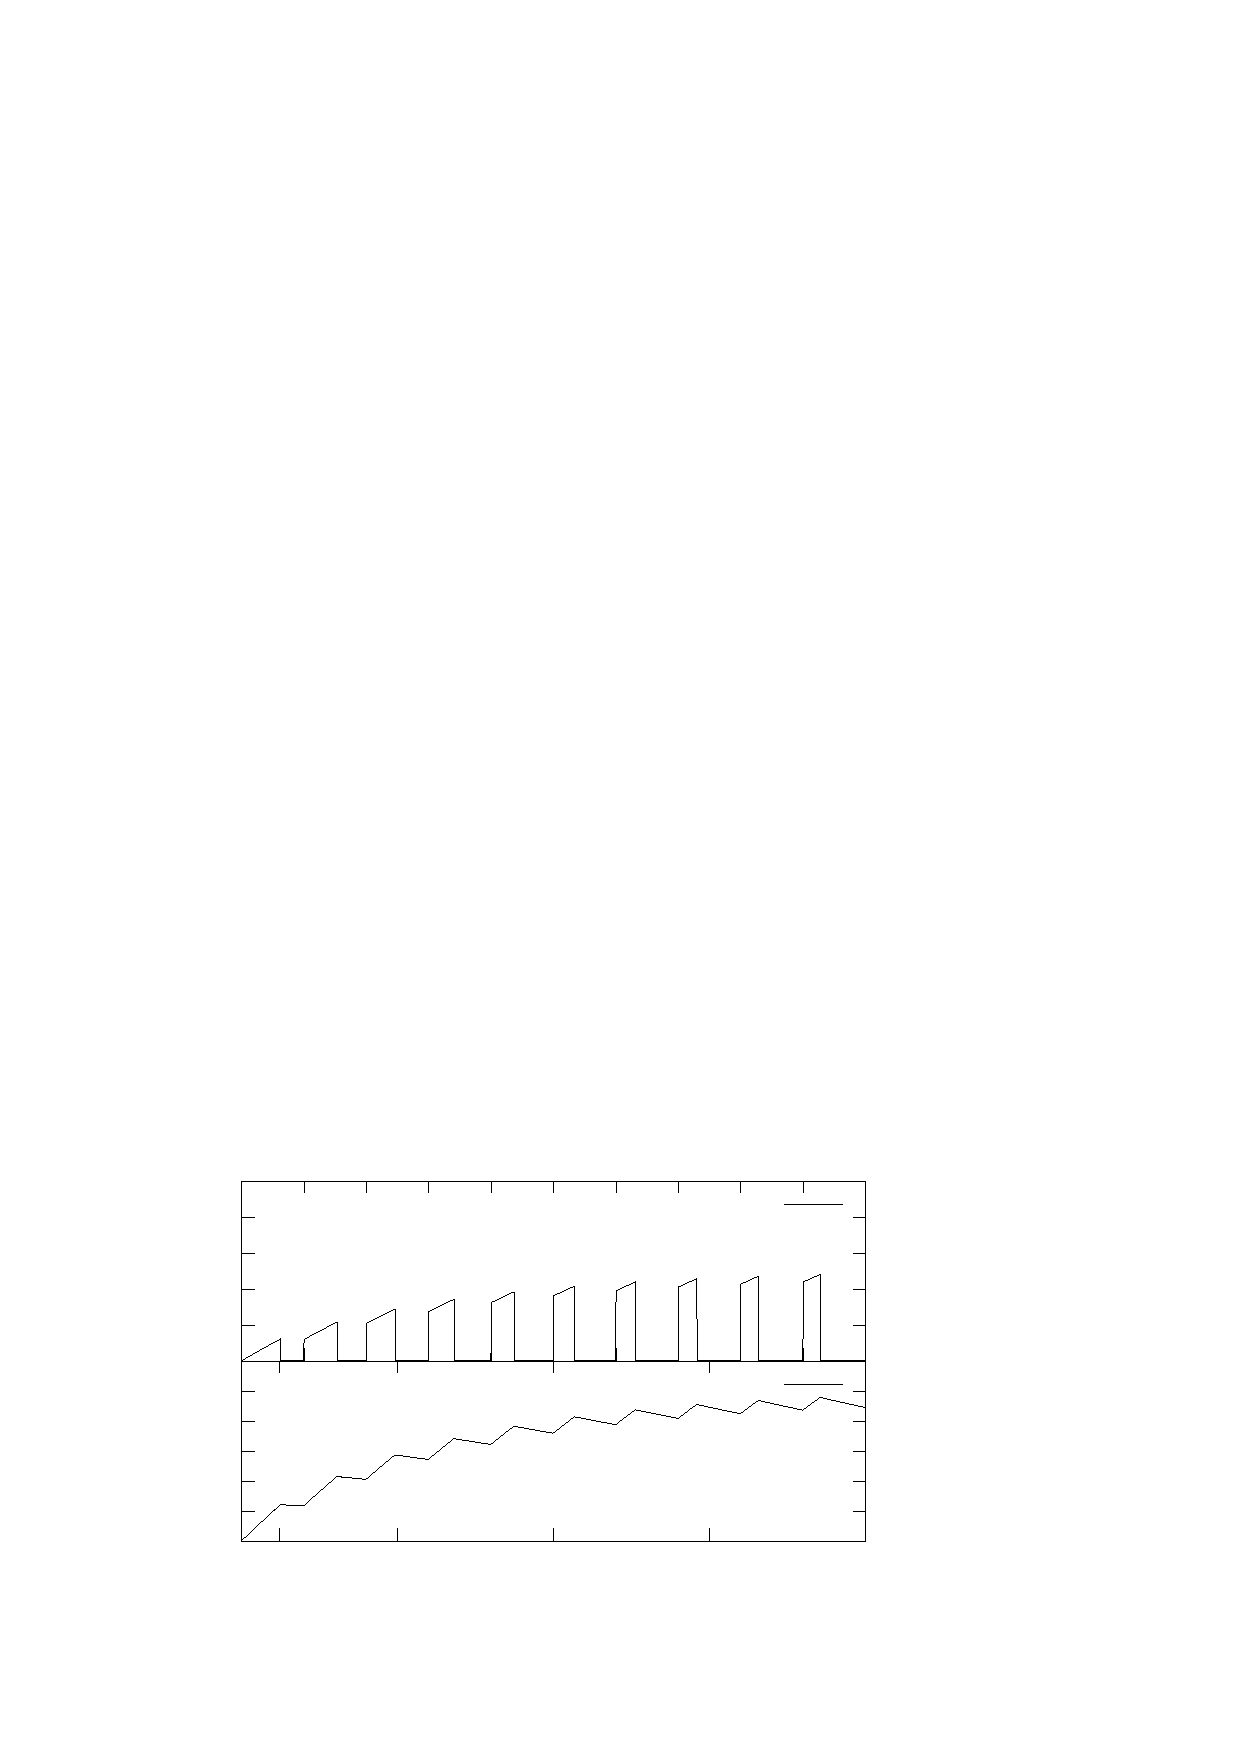
\includegraphics{CS_Siconos}%
\end{picture}%
\begingroup
\setlength{\unitlength}{0.0200bp}%
\begin{picture}(18000,10800)(0,0)%
\put(1925,5832){\makebox(0,0)[r]{\strut{} 0}}%
\put(1925,6696){\makebox(0,0)[r]{\strut{} 2}}%
\put(1925,7560){\makebox(0,0)[r]{\strut{} 4}}%
\put(1925,8424){\makebox(0,0)[r]{\strut{} 6}}%
\put(1925,9288){\makebox(0,0)[r]{\strut{} 8}}%
\put(1925,10152){\makebox(0,0)[r]{\strut{} 10}}%
\put(2200,5282){\makebox(0,0){\strut{}}}%
\put(3697,5282){\makebox(0,0){\strut{}}}%
\put(5195,5282){\makebox(0,0){\strut{}}}%
\put(6692,5282){\makebox(0,0){\strut{}}}%
\put(8190,5282){\makebox(0,0){\strut{}}}%
\put(9687,5282){\makebox(0,0){\strut{}}}%
\put(11185,5282){\makebox(0,0){\strut{}}}%
\put(12682,5282){\makebox(0,0){\strut{}}}%
\put(14180,5282){\makebox(0,0){\strut{}}}%
\put(15677,5282){\makebox(0,0){\strut{}}}%
\put(17175,5282){\makebox(0,0){\strut{}}}%
\put(550,7992){\rotatebox{90}{\makebox(0,0){\strut{}A}}}%
\put(14950,9577){\makebox(0,0)[r]{\strut{}$I_{s}$}}%
\put(1925,1512){\makebox(0,0)[r]{\strut{} 0}}%
\put(1925,2232){\makebox(0,0)[r]{\strut{} 1}}%
\put(1925,2952){\makebox(0,0)[r]{\strut{} 2}}%
\put(1925,3672){\makebox(0,0)[r]{\strut{} 3}}%
\put(1925,4392){\makebox(0,0)[r]{\strut{} 4}}%
\put(1925,5112){\makebox(0,0)[r]{\strut{} 5}}%
\put(1925,5832){\makebox(0,0)[r]{\strut{} 6}}%
\put(17175,962){\makebox(0,0){\strut{}2000}}%
\put(13429,962){\makebox(0,0){\strut{}1500}}%
\put(9684,962){\makebox(0,0){\strut{}1000}}%
\put(5938,962){\makebox(0,0){\strut{}500}}%
\put(3099,962){\makebox(0,0){\strut{}$t_s$}}%
\put(825,3672){\rotatebox{90}{\makebox(0,0){\strut{}V}}}%
\put(9687,137){\makebox(0,0){\strut{}time $micro$ s}}%
\put(14950,5257){\makebox(0,0)[r]{\strut{}$V_2$}}%
\end{picture}%
\endgroup
\endinput
}
  }\hspace{-2mm}
  \subfigure[{\sc Eldo} simulation ]  
  {\label{fig:ELDO_SIMU_CS} 
        \resizebox{0.5\linewidth}{!}{%GNUPLOT: LaTeX picture with Postscript
\begin{picture}(0,0)%
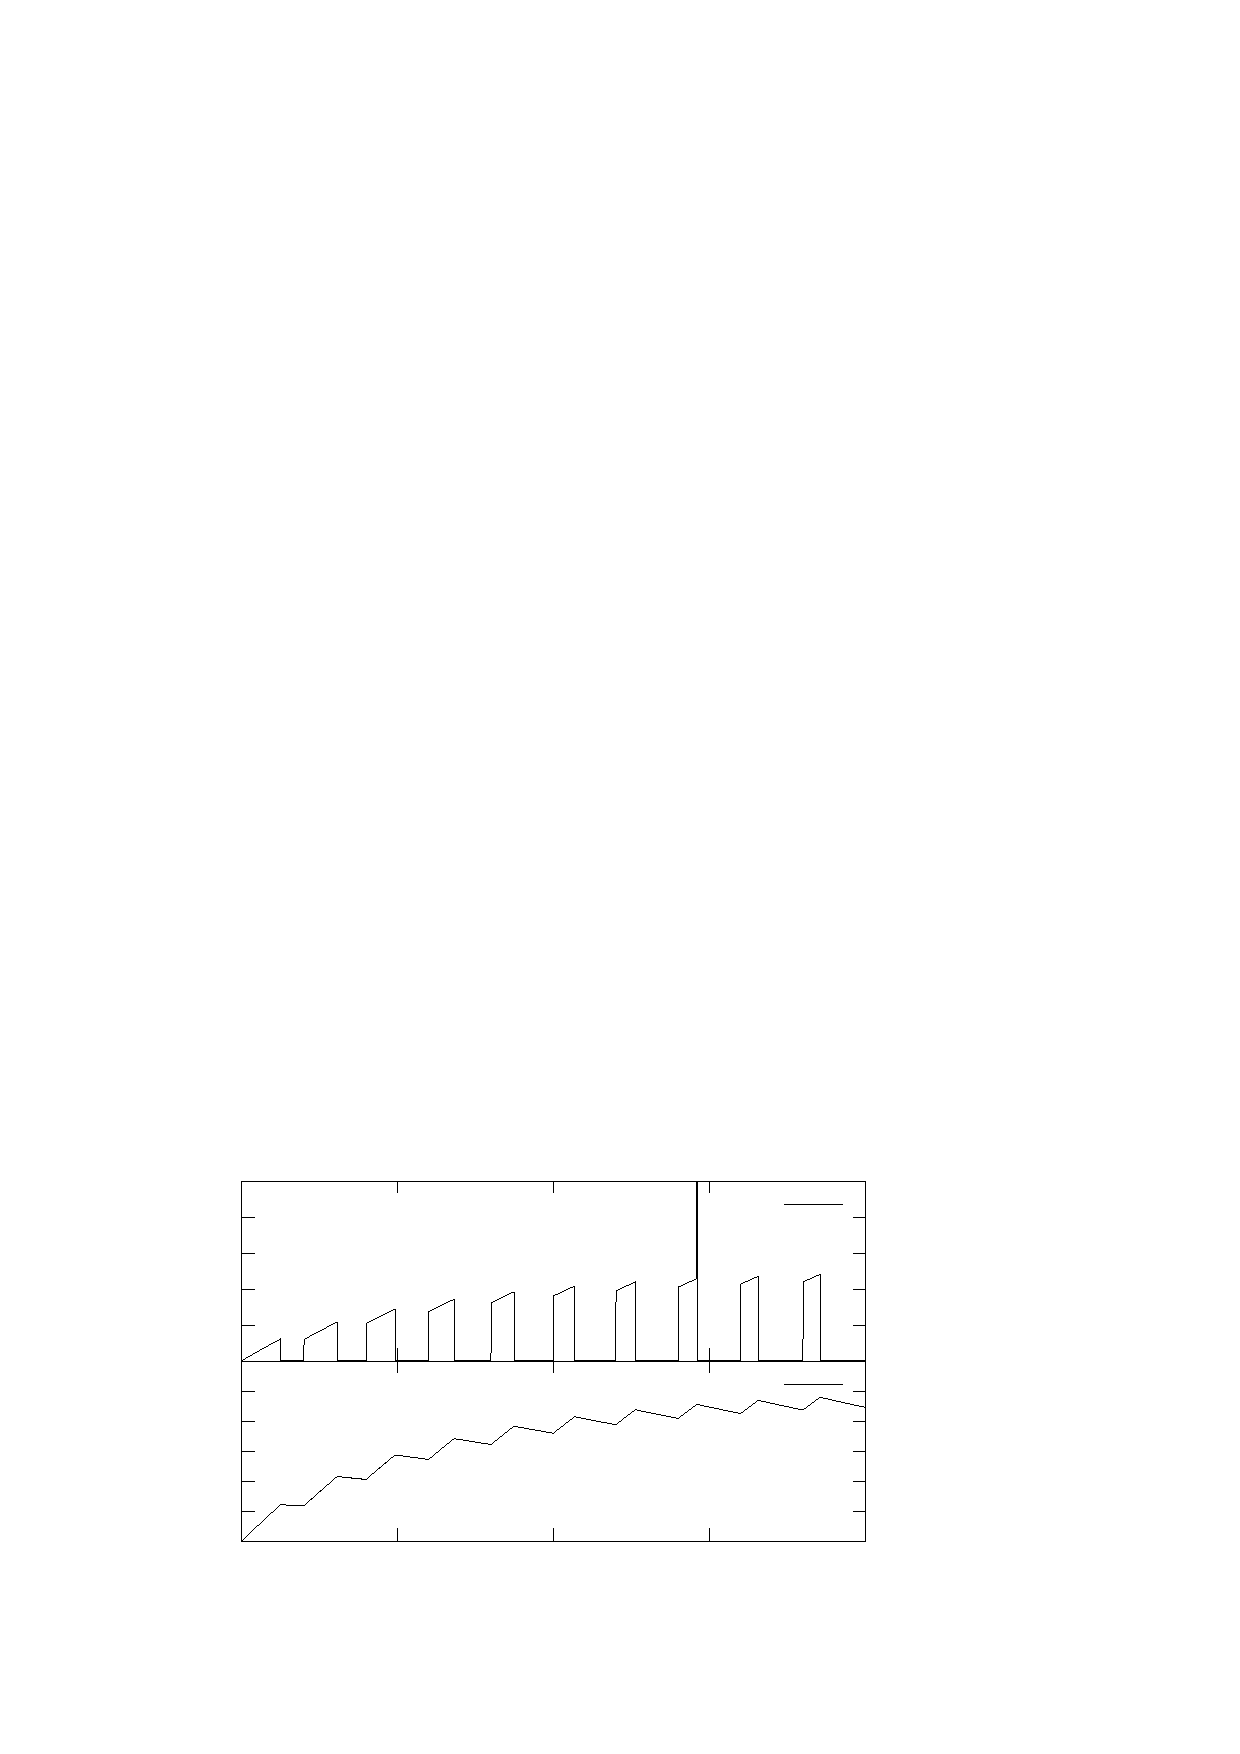
\includegraphics{eldo}%
\end{picture}%
\begingroup
\setlength{\unitlength}{0.0200bp}%
\begin{picture}(18000,10800)(0,0)%
\put(1925,5832){\makebox(0,0)[r]{\strut{} 0}}%
\put(1925,6696){\makebox(0,0)[r]{\strut{} 2}}%
\put(1925,7560){\makebox(0,0)[r]{\strut{} 4}}%
\put(1925,8424){\makebox(0,0)[r]{\strut{} 6}}%
\put(1925,9288){\makebox(0,0)[r]{\strut{} 8}}%
\put(1925,10152){\makebox(0,0)[r]{\strut{} 10}}%
\put(2200,5282){\makebox(0,0){\strut{}}}%
\put(5944,5282){\makebox(0,0){\strut{}}}%
\put(9687,5282){\makebox(0,0){\strut{}}}%
\put(13431,5282){\makebox(0,0){\strut{}}}%
\put(17175,5282){\makebox(0,0){\strut{}}}%
\put(550,7992){\rotatebox{90}{\makebox(0,0){\strut{}A}}}%
\put(14950,9577){\makebox(0,0)[r]{\strut{}$I_R$}}%
\put(1925,1512){\makebox(0,0)[r]{\strut{} 0}}%
\put(1925,2232){\makebox(0,0)[r]{\strut{} 1}}%
\put(1925,2952){\makebox(0,0)[r]{\strut{} 2}}%
\put(1925,3672){\makebox(0,0)[r]{\strut{} 3}}%
\put(1925,4392){\makebox(0,0)[r]{\strut{} 4}}%
\put(1925,5112){\makebox(0,0)[r]{\strut{} 5}}%
\put(1925,5832){\makebox(0,0)[r]{\strut{} 6}}%
\put(2200,962){\makebox(0,0){\strut{}0}}%
\put(5944,962){\makebox(0,0){\strut{}500}}%
\put(9687,962){\makebox(0,0){\strut{}1000}}%
\put(13431,962){\makebox(0,0){\strut{}1500}}%
\put(17175,962){\makebox(0,0){\strut{}2000}}%
\put(825,3672){\rotatebox{90}{\makebox(0,0){\strut{}V}}}%
\put(9687,137){\makebox(0,0){\strut{}time $micro$ s}}%
\put(14950,5257){\makebox(0,0)[r]{\strut{}$V_2$}}%
\end{picture}%
\endgroup
\endinput
}
  } 
 \caption{Switched circuit simulations.}
\label{figSimuCS}
\end{figure*}


\begin{remark}
In \cite{maffezzoni2006} an event-driven numerical method is proposed to solve the non convergence issue. However it is reliable only if the switching times can be precisely estimated, a shortcoming not encountered  with the NSDS and the  Moreau's time-stepping method. 
\end{remark}

\subsection{Numerical results with {\sc Eldo}}
{\sc Eldo} does not provide any non--smooth switch model. But it furnishes the 'VSWITCH' one described in
(\ref{eq:eldo_switch}), where  $R_S$ is the controlled resistor value of the switch, and $V_{C}$ the voltage
control. Setting $V_{\off}$ to $0$, and choosing a small value for $V_{\on}$ lead to:


  \begin{equation}
    \label{eq:eldo_switch}
    R_S(t)=\begin{cases}R_\on\; & \mbox{if}\;V_{C}(t) \geq V_{\on} \\   R_\off\;  & \mbox{if}\;V_{C}(t) \leq
%    V_{\off} \\ (V_{C}(R_\off\;-R_\on\;)+ R_\on\; V_{\off}- \\ \qquad R_\off\;V_{\on})/(V_{\off}-V_{\on})& \mbox{if}\;V_{\off}<V_{C}(t) < V_{\on} \end{cases}
    V_{off} \\ (V_{C}(t)(R_\off\;-R_\on\;)+ R_\on\; V_{\off}- \\ \qquad
    R_\off\;V_{\on})/(V_{\off}-V_{\on})& \mbox{otherwise}\; \end{cases}
  \end{equation}
  which is close to \eqref{switchmodel1} for the chosen parameters. \\Simulations have been done using
  different sets of parameters. It is noteworthy that the
behavior of {\sc Eldo} depends on these values. For example, using a Backward Euler with the time step fixed to $0.1 \micro \second$ and $V_{on}=1e-4\volt$, $V_{off}=0 \volt$,
$R_\off\; = 1000 \ohm$, $R_\on\;=0.001\ohm$ cause troubles during the {\sc Eldo}
simulation, some messages like 'Newton no-convergence' appear. Fig.~\ref{fig:ELDO_SIMU_CS}
  shows the {\sc Eldo} simulation. The values are very close to the {\sc Siconos} simulation, except for the steps corresponding to the
  no-convergence messages. In this case, the resulting current value is absurd. \\



This academic example demonstrates that analog tools can fail to simulate a switched circuit.

\section{Results on the buck converter}
\label{section4}


\begin{figure*}[!ht]
\centerline{
 \scalebox{1.0}{
    \input{./figure/buck.pstex_t}
 }
}
\caption{Buck converter}
\label{fig-Buck-converter}
\end{figure*}
The components are modelled with either linear, or piecewise linear, or set-valued relations yielding a nonsmooth dynamical system of the linear time invariant complementarity systems class. The features of the models are given thereafter.

\paragraph{Power MOSFETS pMOS/nMOS} they are described as an assembly of a
piecewise-linear current source $I_{DS} = f(V_{GS}, V_{DS})$ and the intrinsic diode
(DpMOS and DnMOS) with an ideal characteristic.
The capacitances were not taken into account. The diodes residual voltage is
$1\volt$. 
The MOSFETs transconductance KP was set to $10 \ampere\volt^{-2}$ and
their threshold voltage to respectively $V_T = -2 \volt$ for the pMOS and $V_T= 2 \volt$ for
the nMOS. One can notice that the sum of their absolute values largely
exceeds the supply voltage $V_{I} = 3 \volt$ , thus providing non-overlapping
conduction times. The other physical parameters as chosen as follows : $\mu = 750~cm^2.\volt^{-1}.\second^{-1}$ for a nMOS and $\mu=250~cm^2.\volt^{-1}.\second^{-1}$ for a pMOS, $\epsilon_{Ox} = \epsilon_{r~SiO_2} \cdot \epsilon_0$ with $\epsilon_{r~SiO_2} \approx 3.9$, $t_{OX} \approx 4 \nano\meter$ $W = 130\nano \meter$ $L=180 \nano\meter$. 

The piecewise linear model uses $6$ segments given by the following data: $ c_1 = 0.09 , c_2=0.2238 ,
c_3=0.4666 , c_4=1.1605 , c_5=2.8863,  a_1 = 0 , a_2=0.1, a_3=0.2487 , a_4=0.6182 , a_5=1.5383$. The
relative error between $f(\cdot)$ and $f_\pwl(\cdot)$ is kept below $0.1$ for $0.1 \leq x < 3.82$.
The absolute error is less than $2 \cdot 10^{-3}$ for $0 \leq x < 0.1$ and $0$ for negative $x$. In
practice, the values of $V_G,V_S,V_D,V_T$ in logic integrated circuits allow  a good approximation
of $f(\cdot)$ by $f_\pwl(\cdot)$. 


\paragraph{Compensator amplifier} it is modelled as a $1.10^5$ gain and an output low-pass
filter with a cutoff frequency of $30 \mega\hertz$.
\paragraph{Comparator} it is modelled as a piecewise-linear function whose value is $0$ if
$x < -0.15\volt$ and 3 if $x > 0.15\volt$.
\paragraph{Ramp voltage} the frequency is $600 \kilo\hertz$ and the bounds are $0$ and $0.75 V_I = 2.25 \volt$ .
The rise time is $1.655 \nano\second$ and the fall time is $10 \nano\second$.
\paragraph{Standard values for other components} $V_I = 3 \volt , L = 10 \micro\henry, C = 22 \micro \farad, R_{load} =
10\ohm , R_{11} = 15.58 \kilo \ohm , R_{12} = 227.8 \kilo \ohm ,R_{21} = 5.613 \mega \ohm, C_{11} = 20 \pico \farad, C_{21} =
1.9 \pico \farad$.
\paragraph{Values exhibiting a sliding mode}$L = 4 \micro \henry, C =
10 \micro \farad, R_{11} = 10 \kilo \ohm , R_{21}= 8 \mega \ohm, C_{11} = 10 \pico \farad$.

The reference voltage Vref rises from 0 to 1.8 V in 0.1 ms at the beginning
of the simulation.
The output voltage Voutput is regulated to track the reference voltage $V_{ref}$ when
$V_I$ or $V_{ref}$ or the load current vary. The error voltage Verror is a filtered value
of the difference between Voutput and Vref . This voltage signal is converted
into a time length thanks to a comparison with the periodic ramp signal. The
comparator drives the pMOS transistor which in turn provides more or less
charge to the output depending on the error level. The operation of a buck
converter involves both a relatively slow dynamics when the switching elements
(MOS and diodes) are keeping their conducting state, and a fast dynamics when
the states change. The orders of magnitude are $ 50 \pico \second$ for some switching details,
$1 \micro \second$ for a slow variation period and $100 \micro \second$ at least for a settling period of the
whole circuit requiring a simulation.

\subsection{The dynamical equations}
\label{section41}
The nonsmooth DAE has been generated using the automatic circuit equation formulation described in
Section~\ref{sec:acef}. It leads to a dynamical system with 25 states coupled to an inclusion rule.
The dimension of the inclusion rule is $24$.  

\subsection{Numerical results with {\sc Siconos},  and comparisons}
\label{section42}
\subsubsection{Simulation with {\sc Siconos}}
 The start-up of the converter was simulated thanks to {\sc Siconos}. As initial conditions, all state variables are zeroed.
The detailed analysis of the switching events requires to use a time step as
small as $50 \pico \second$. The simulations are carried with a fixed time step, $4.10^{6}$ steps
are then computed for the $200 \micro \second$ long settling of the output voltage. The OSNSP
solvers used are PATH with a convergence tolerance of $1e-7$, and a semi-smooth Newton method based on the Fischer-Bursmeister
reformulation\cite{Deluca.ea1996} that is our own implementation using a convergence tolerance of $1e-12$.
The overall result is shown on the Fig.~\ref{fig:figSimuBuck}.  


{\bf Simulation time:} The CPU time required to achieve the simulation is $60 \second$ on a
Pentium 4 processor clocked at 3 GHz. It includes $19 \second$ in the MLCP solvers, $40 \second$ in
matrices products. The time to export the resulting data is not included.


\begin{figure*}[!ht]
  \subfigure[$V_{load}$ ]{\label{fig:SICONOS_SIMU_BUCK_VLOAD}
        \resizebox{0.5\linewidth}{!}{%GNUPLOT: LaTeX picture with Postscript
\begin{picture}(0,0)%
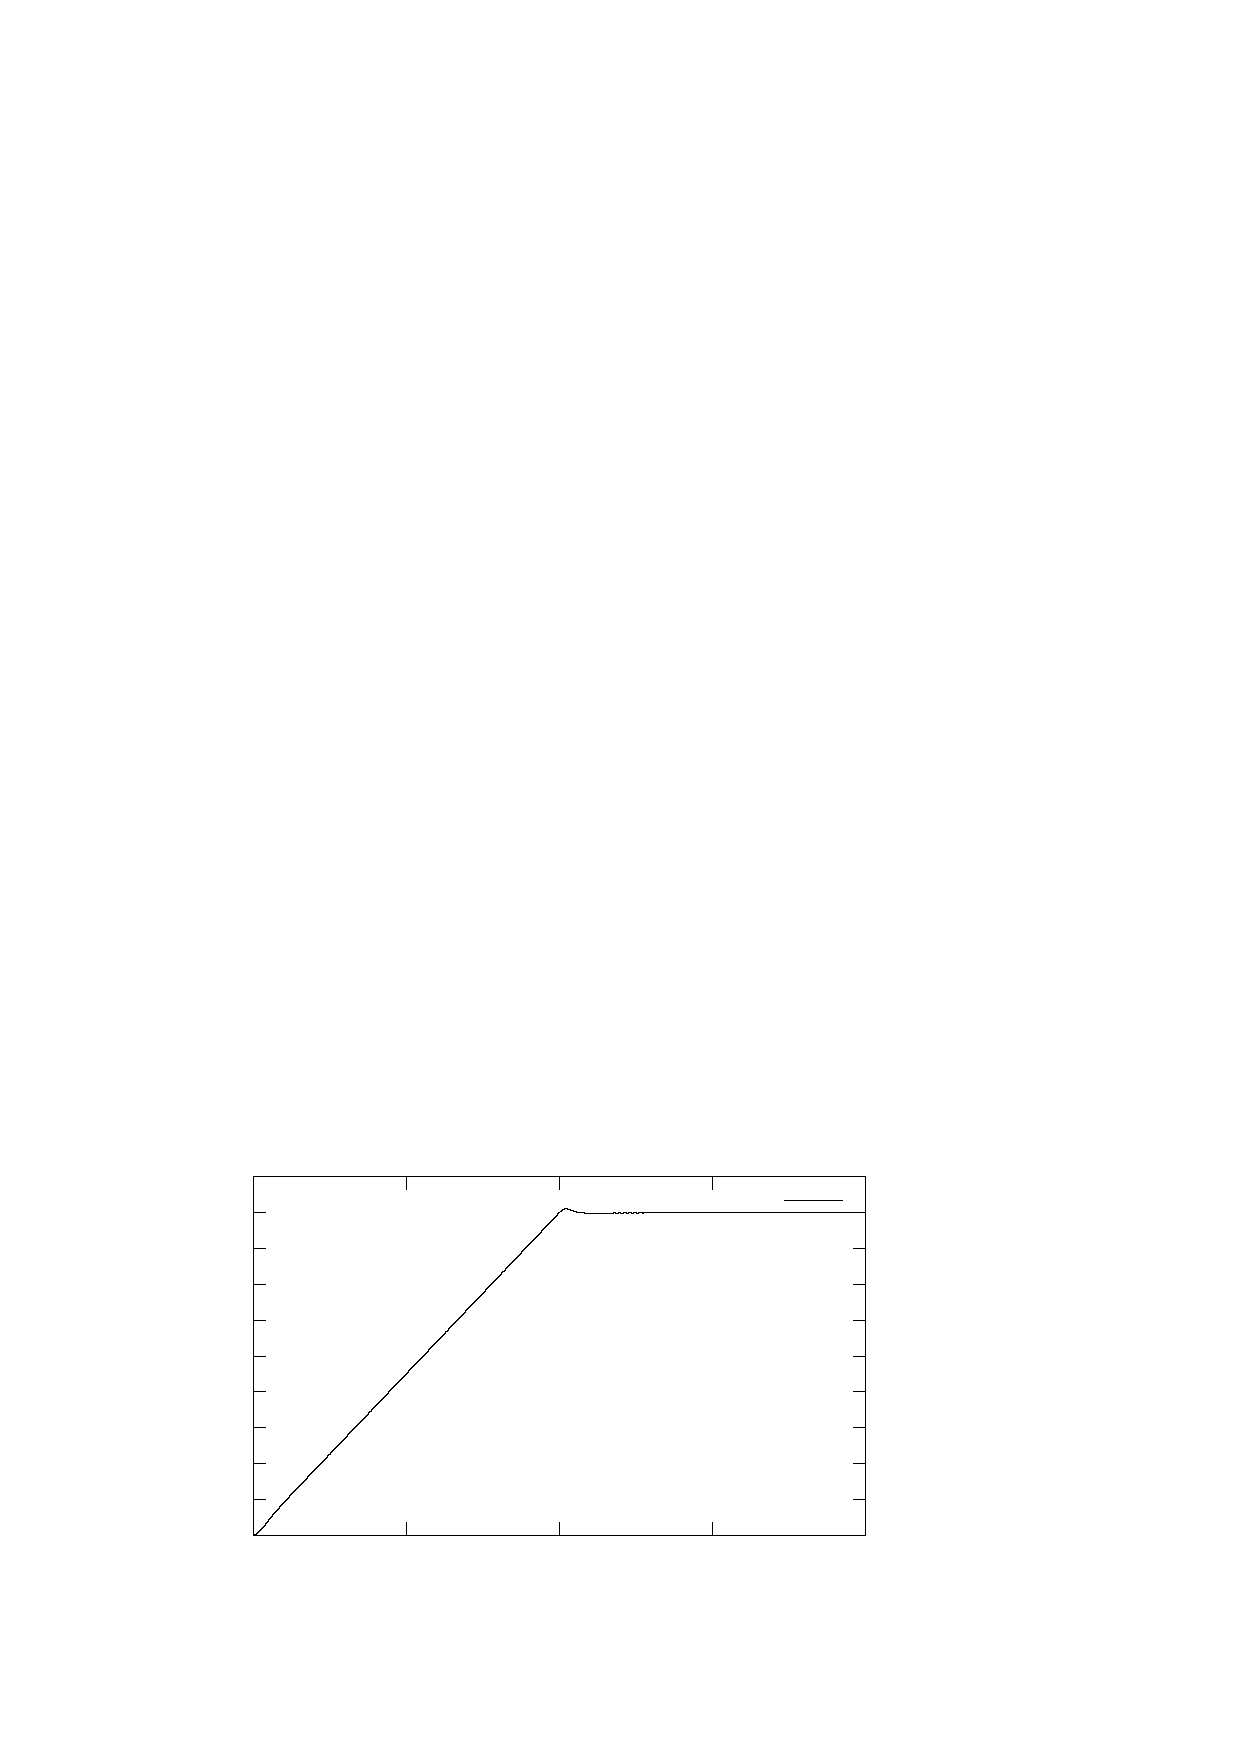
\includegraphics{Vload}%
\end{picture}%
\begingroup
\setlength{\unitlength}{0.0200bp}%
\begin{picture}(18000,10800)(0,0)%
\put(2200,1650){\makebox(0,0)[r]{\strut{} 0}}%
\put(2200,2510){\makebox(0,0)[r]{\strut{} 0.2}}%
\put(2200,3370){\makebox(0,0)[r]{\strut{} 0.4}}%
\put(2200,4230){\makebox(0,0)[r]{\strut{} 0.6}}%
\put(2200,5090){\makebox(0,0)[r]{\strut{} 0.8}}%
\put(2200,5950){\makebox(0,0)[r]{\strut{} 1}}%
\put(2200,6810){\makebox(0,0)[r]{\strut{} 1.2}}%
\put(2200,7670){\makebox(0,0)[r]{\strut{} 1.4}}%
\put(2200,8530){\makebox(0,0)[r]{\strut{} 1.6}}%
\put(2200,9390){\makebox(0,0)[r]{\strut{} 1.8}}%
\put(2200,10250){\makebox(0,0)[r]{\strut{} 2}}%
\put(2475,1100){\makebox(0,0){\strut{} 0}}%
\put(6150,1100){\makebox(0,0){\strut{} 50}}%
\put(9825,1100){\makebox(0,0){\strut{} 100}}%
\put(13500,1100){\makebox(0,0){\strut{} 150}}%
\put(17175,1100){\makebox(0,0){\strut{} 200}}%
\put(550,5950){\rotatebox{90}{\makebox(0,0){\strut{}V}}}%
\put(9825,275){\makebox(0,0){\strut{}time $\micro s$}}%
\put(14950,9675){\makebox(0,0)[r]{\strut{}$V_{load}$}}%
\end{picture}%
\endgroup
\endinput
}
  }\hspace{-2mm}
  \subfigure[$I_L$]  
  {\label{fig:SICONOS_SIMU_BUCK_IL} 
        \resizebox{0.5\linewidth}{!}{%GNUPLOT: LaTeX picture with Postscript
\begin{picture}(0,0)%
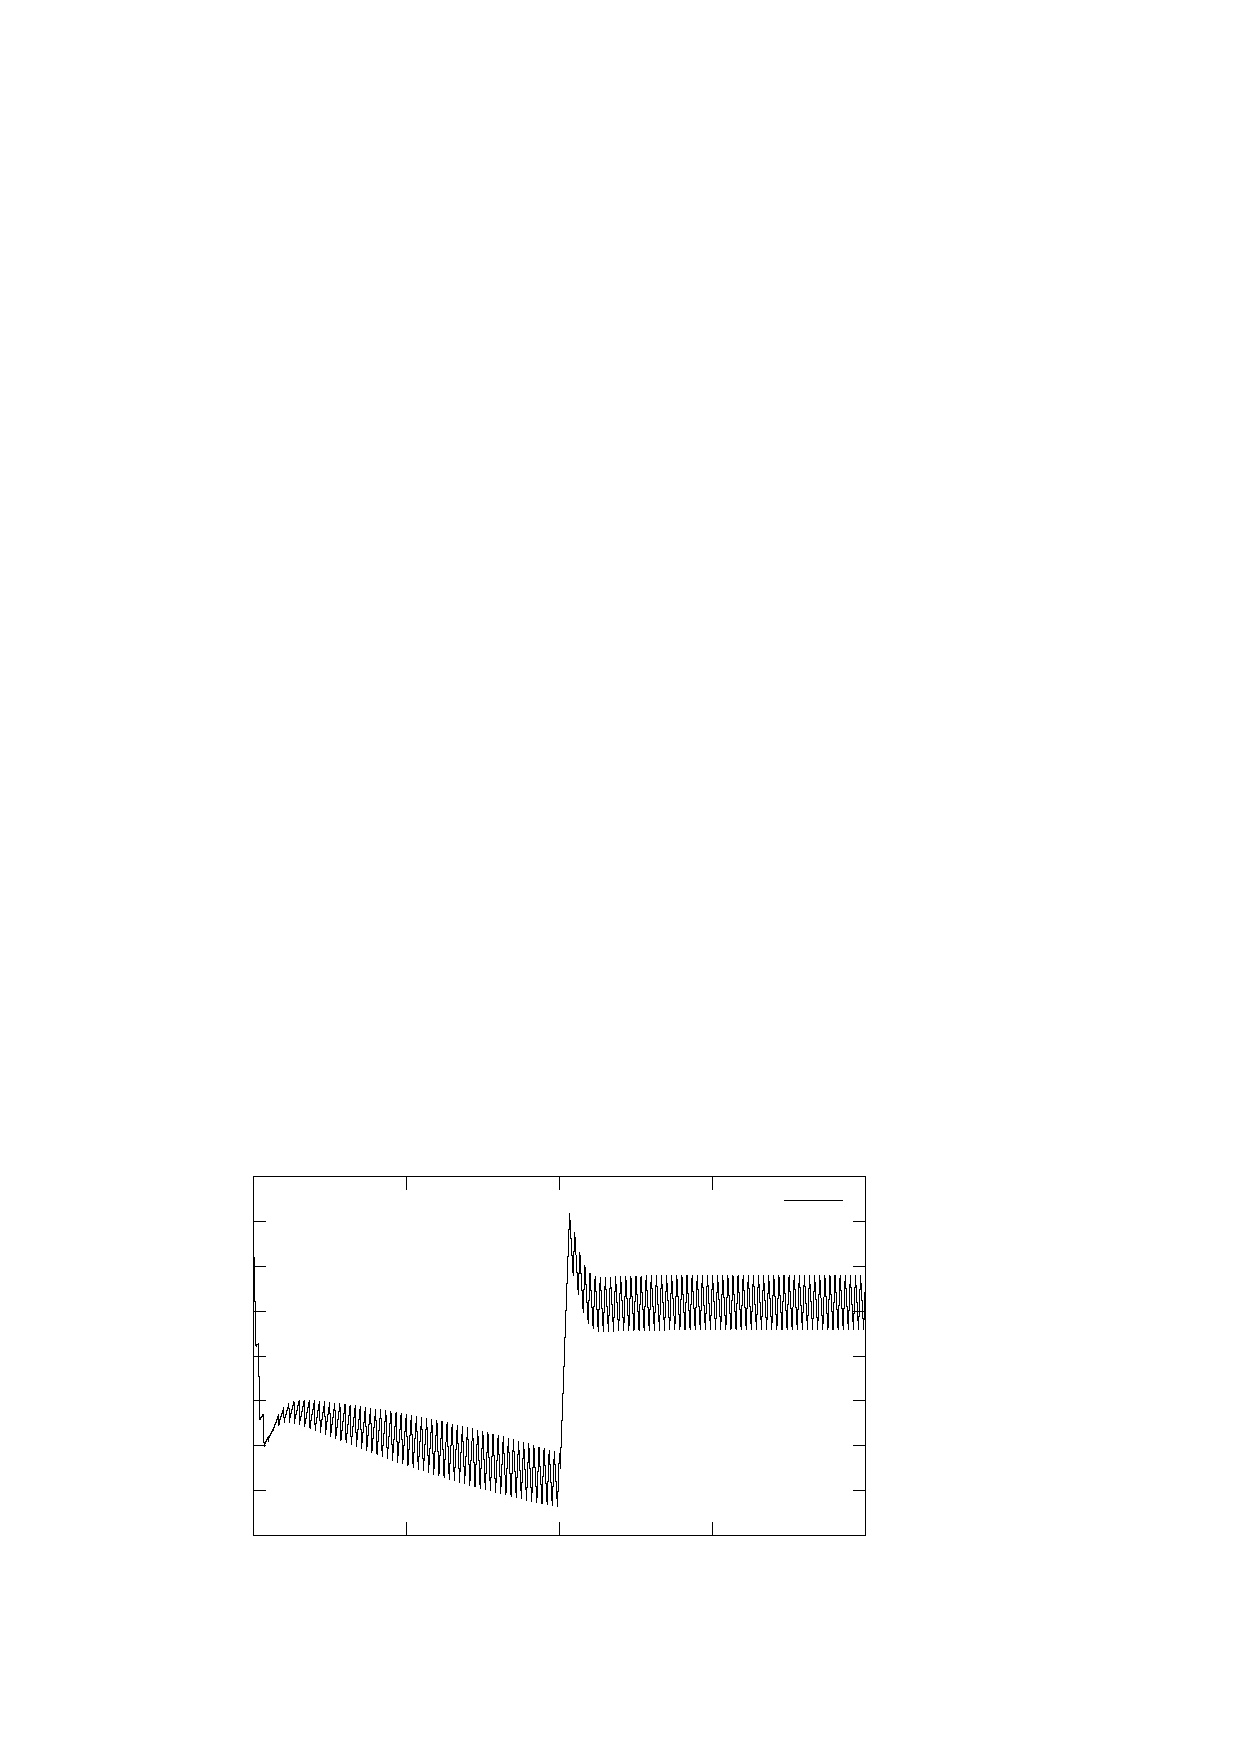
\includegraphics{Il}%
\end{picture}%
\begingroup
\setlength{\unitlength}{0.0200bp}%
\begin{picture}(18000,10800)(0,0)%
\put(2200,1650){\makebox(0,0)[r]{\strut{}-0.7}}%
\put(2200,2725){\makebox(0,0)[r]{\strut{}-0.6}}%
\put(2200,3800){\makebox(0,0)[r]{\strut{}-0.5}}%
\put(2200,4875){\makebox(0,0)[r]{\strut{}-0.4}}%
\put(2200,5950){\makebox(0,0)[r]{\strut{}-0.3}}%
\put(2200,7025){\makebox(0,0)[r]{\strut{}-0.2}}%
\put(2200,8100){\makebox(0,0)[r]{\strut{}-0.1}}%
\put(2200,9175){\makebox(0,0)[r]{\strut{} 0}}%
\put(2200,10250){\makebox(0,0)[r]{\strut{} 0.1}}%
\put(2475,1100){\makebox(0,0){\strut{} 0}}%
\put(6150,1100){\makebox(0,0){\strut{} 50}}%
\put(9825,1100){\makebox(0,0){\strut{} 100}}%
\put(13500,1100){\makebox(0,0){\strut{} 150}}%
\put(17175,1100){\makebox(0,0){\strut{} 200}}%
\put(550,5950){\rotatebox{90}{\makebox(0,0){\strut{}A}}}%
\put(9825,275){\makebox(0,0){\strut{}time $\micro s$}}%
\put(14950,9675){\makebox(0,0)[r]{\strut{}$I_L$}}%
\end{picture}%
\endgroup
\endinput
}
  } \\
  \subfigure[pMOS drain potential]  
  {\label{fig:SICONOS_SIMU_BUCK_MOS} 
        \resizebox{0.5\linewidth}{!}{%GNUPLOT: LaTeX picture with Postscript
\begin{picture}(0,0)%
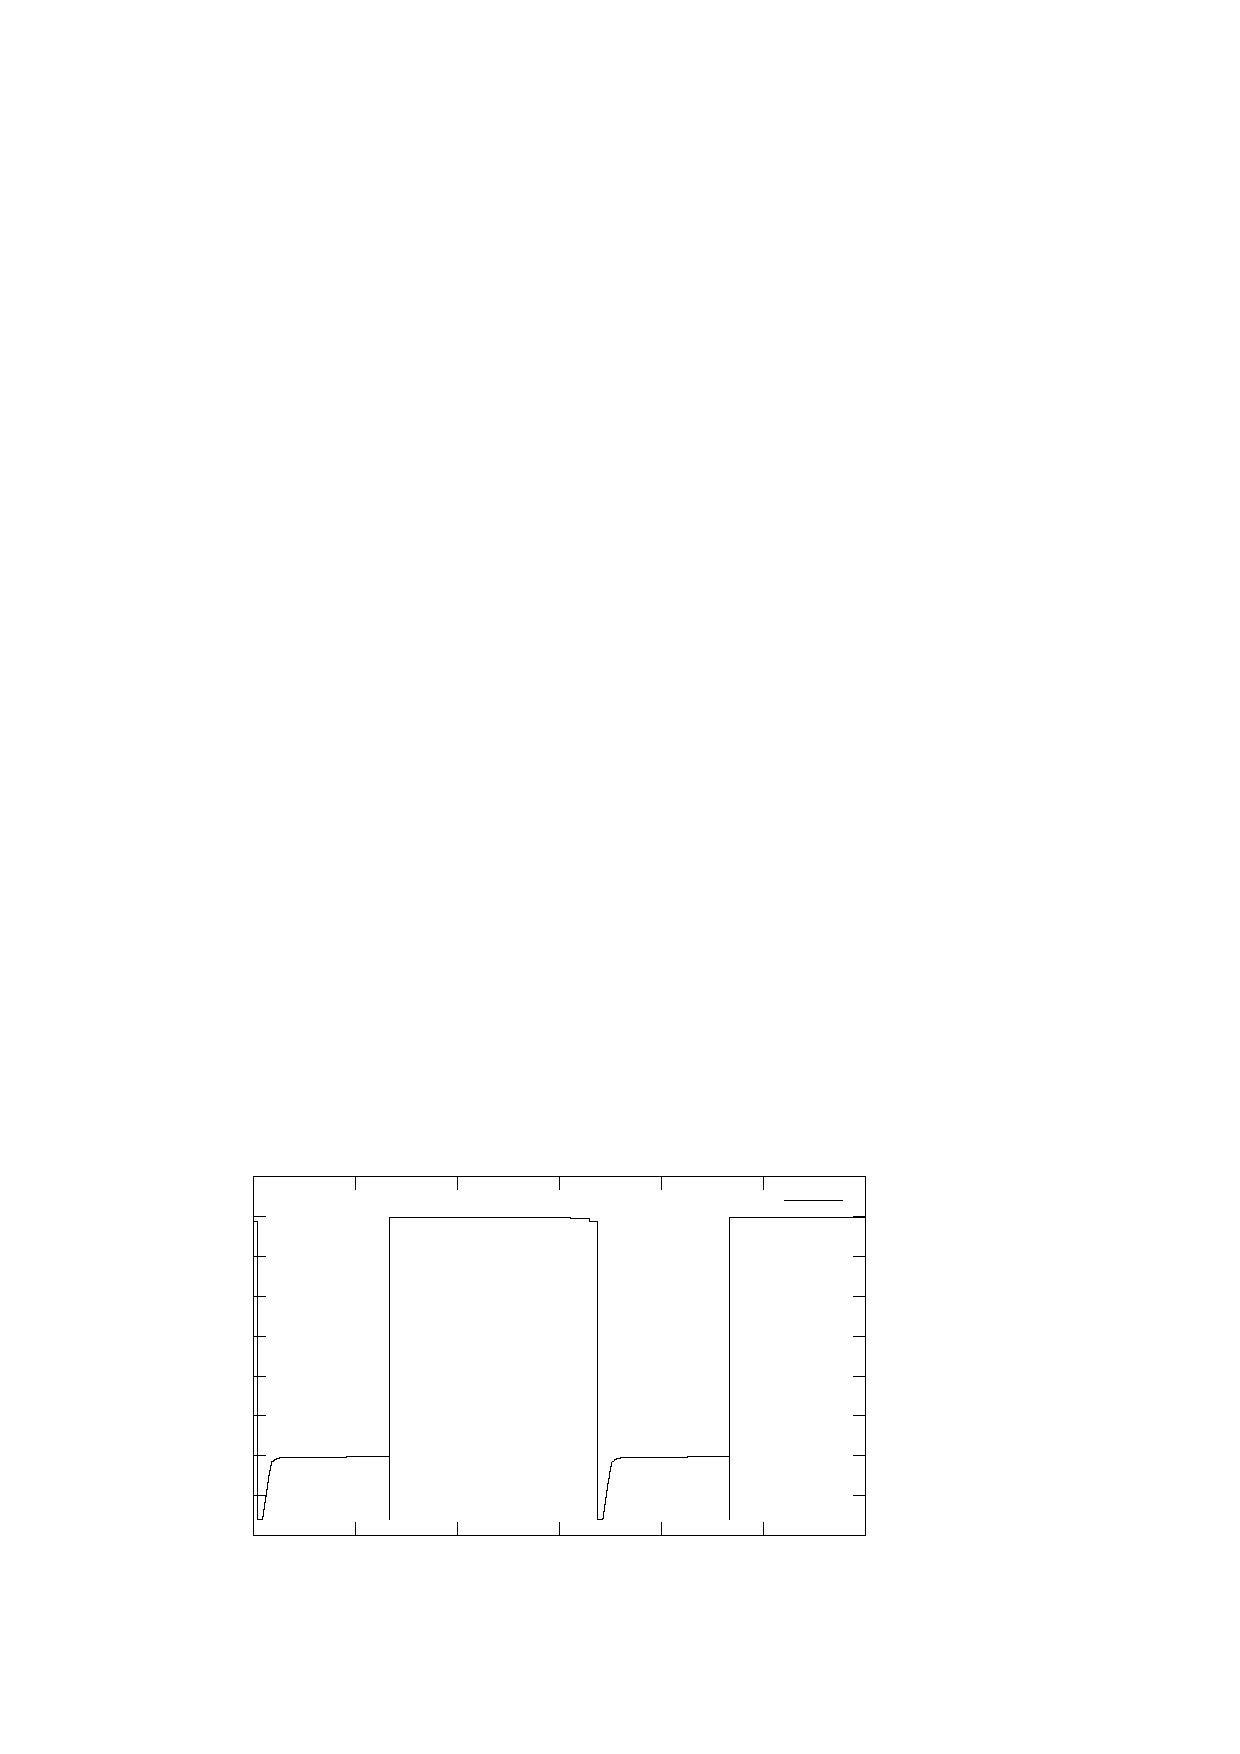
\includegraphics{MOSPdrain}%
\end{picture}%
\begingroup
\setlength{\unitlength}{0.0200bp}%
\begin{picture}(18000,10800)(0,0)%
\put(2200,1650){\makebox(0,0)[r]{\strut{}-1}}%
\put(2200,2606){\makebox(0,0)[r]{\strut{}-0.5}}%
\put(2200,3561){\makebox(0,0)[r]{\strut{} 0}}%
\put(2200,4517){\makebox(0,0)[r]{\strut{} 0.5}}%
\put(2200,5472){\makebox(0,0)[r]{\strut{} 1}}%
\put(2200,6428){\makebox(0,0)[r]{\strut{} 1.5}}%
\put(2200,7383){\makebox(0,0)[r]{\strut{} 2}}%
\put(2200,8339){\makebox(0,0)[r]{\strut{} 2.5}}%
\put(2200,9294){\makebox(0,0)[r]{\strut{} 3}}%
\put(2200,10250){\makebox(0,0)[r]{\strut{} 3.5}}%
\put(2475,1100){\makebox(0,0){\strut{} 196}}%
\put(4925,1100){\makebox(0,0){\strut{} 196.5}}%
\put(7375,1100){\makebox(0,0){\strut{} 197}}%
\put(9825,1100){\makebox(0,0){\strut{} 197.5}}%
\put(12275,1100){\makebox(0,0){\strut{} 198}}%
\put(14725,1100){\makebox(0,0){\strut{} 198.5}}%
\put(17175,1100){\makebox(0,0){\strut{} 199}}%
\put(550,5950){\rotatebox{90}{\makebox(0,0){\strut{}V}}}%
\put(9825,275){\makebox(0,0){\strut{}time \micro s}}%
\put(14950,9675){\makebox(0,0)[r]{\strut{}MOS P drain}}%
\end{picture}%
\endgroup
\endinput
}
  }\hspace{-2mm}
  \subfigure[$V_{ramp}$ and $V_{error}$]  
  {\label{fig:SICONOS_SIMU_BUCK_VERROR} 
        \resizebox{0.5\linewidth}{!}{%GNUPLOT: LaTeX picture with Postscript
\begin{picture}(0,0)%
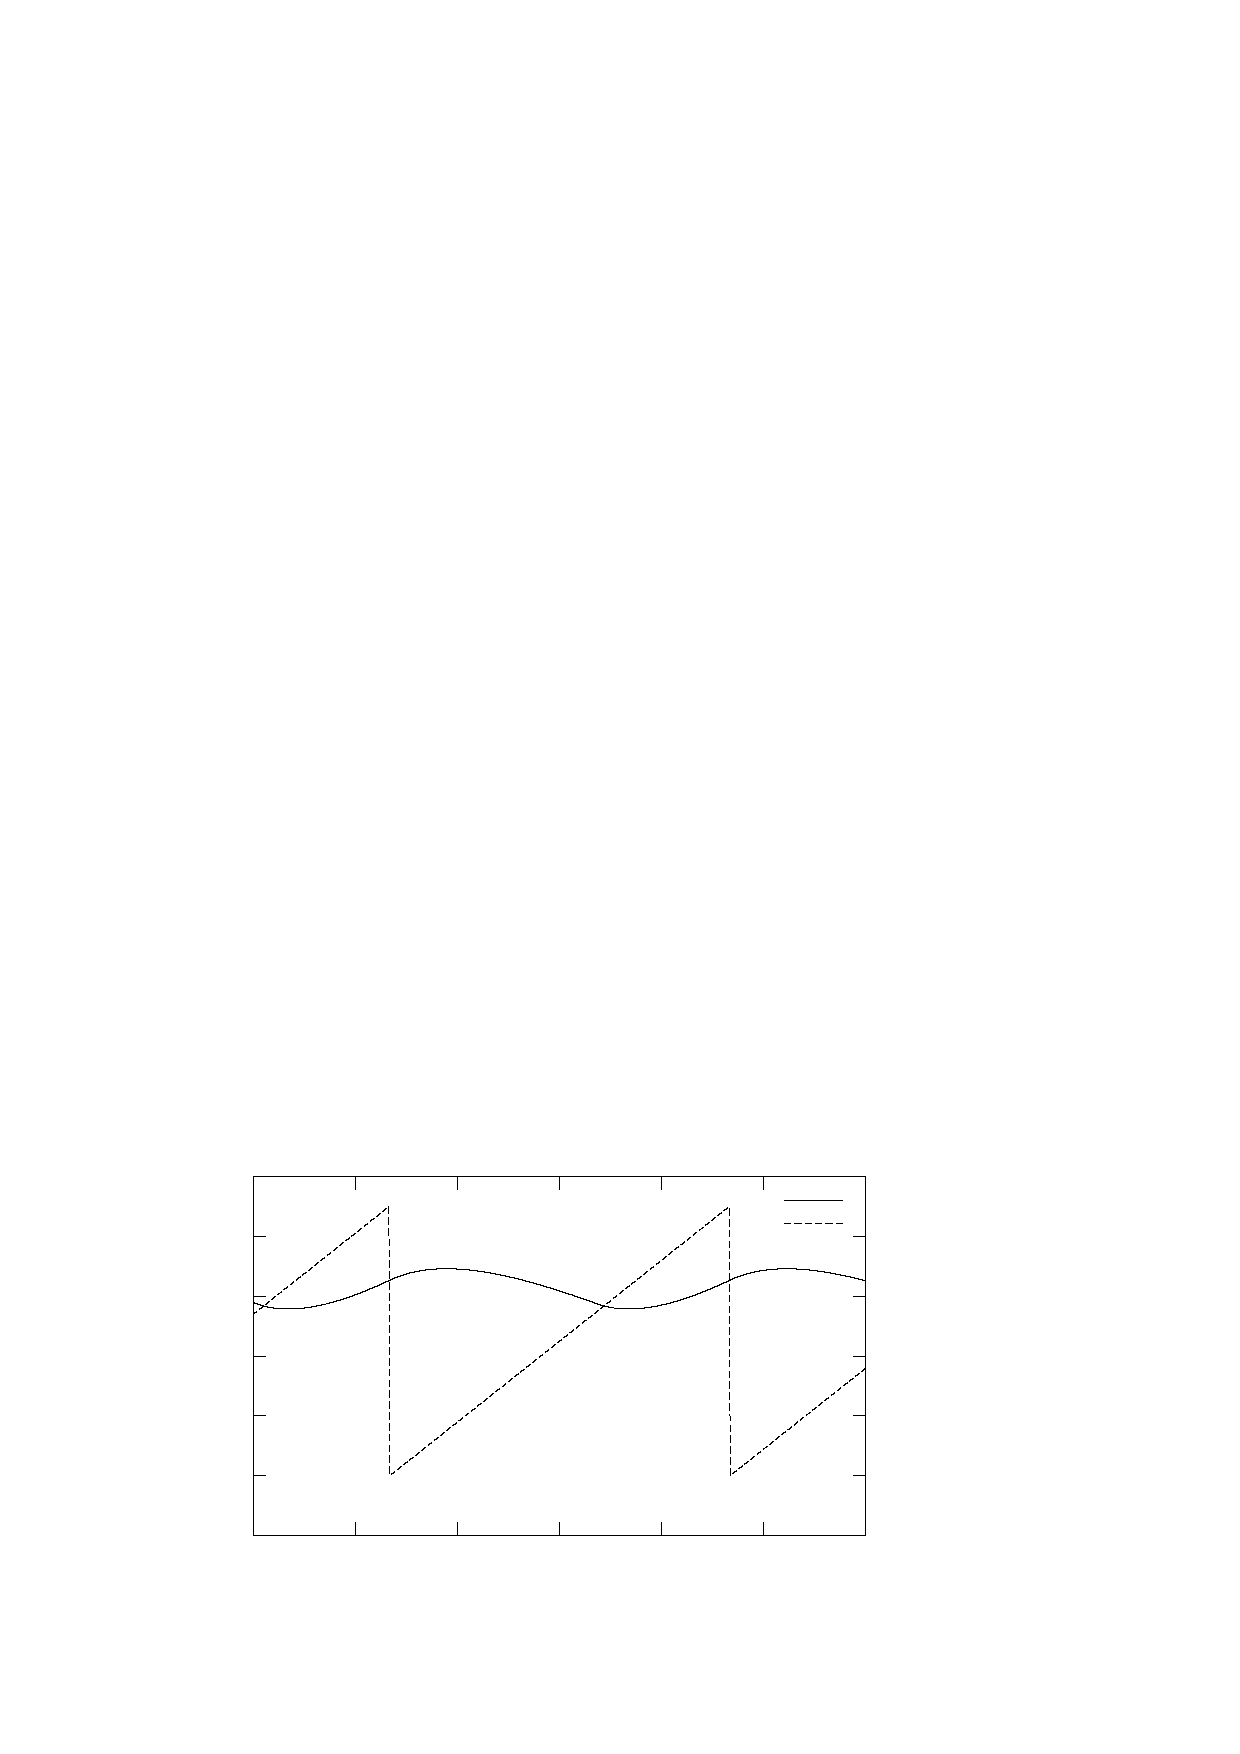
\includegraphics{VrampVerror}%
\end{picture}%
\begingroup
\setlength{\unitlength}{0.0200bp}%
\begin{picture}(18000,10800)(0,0)%
\put(2200,1650){\makebox(0,0)[r]{\strut{}-0.5}}%
\put(2200,3083){\makebox(0,0)[r]{\strut{} 0}}%
\put(2200,4517){\makebox(0,0)[r]{\strut{} 0.5}}%
\put(2200,5950){\makebox(0,0)[r]{\strut{} 1}}%
\put(2200,7383){\makebox(0,0)[r]{\strut{} 1.5}}%
\put(2200,8817){\makebox(0,0)[r]{\strut{} 2}}%
\put(2200,10250){\makebox(0,0)[r]{\strut{} 2.5}}%
\put(2475,1100){\makebox(0,0){\strut{} 196}}%
\put(4925,1100){\makebox(0,0){\strut{} 196.5}}%
\put(7375,1100){\makebox(0,0){\strut{} 197}}%
\put(9825,1100){\makebox(0,0){\strut{} 197.5}}%
\put(12275,1100){\makebox(0,0){\strut{} 198}}%
\put(14725,1100){\makebox(0,0){\strut{} 198.5}}%
\put(17175,1100){\makebox(0,0){\strut{} 199}}%
\put(550,5950){\rotatebox{90}{\makebox(0,0){\strut{}V}}}%
\put(9825,275){\makebox(0,0){\strut{}time \micro s}}%
\put(14950,9675){\makebox(0,0)[r]{\strut{}$V_{error}$}}%
\put(14950,9125){\makebox(0,0)[r]{\strut{}$V_{ramp}$}}%
\end{picture}%
\endgroup
\endinput
}
  } 
 \caption{{\sc Siconos} buck simulation using standard parameters.}
\label{fig:figSimuBuck}
\end{figure*}
\begin{figure*}[!ht]
    \subfigure[$V_{comp}$ and $V_{drain}$]  
  {\label{fig:SICONOS_SIMU_BUCK_SLIDING_MOS_COMP} 
        \resizebox{0.5\linewidth}{!}{%GNUPLOT: LaTeX picture with Postscript
\begin{picture}(0,0)%
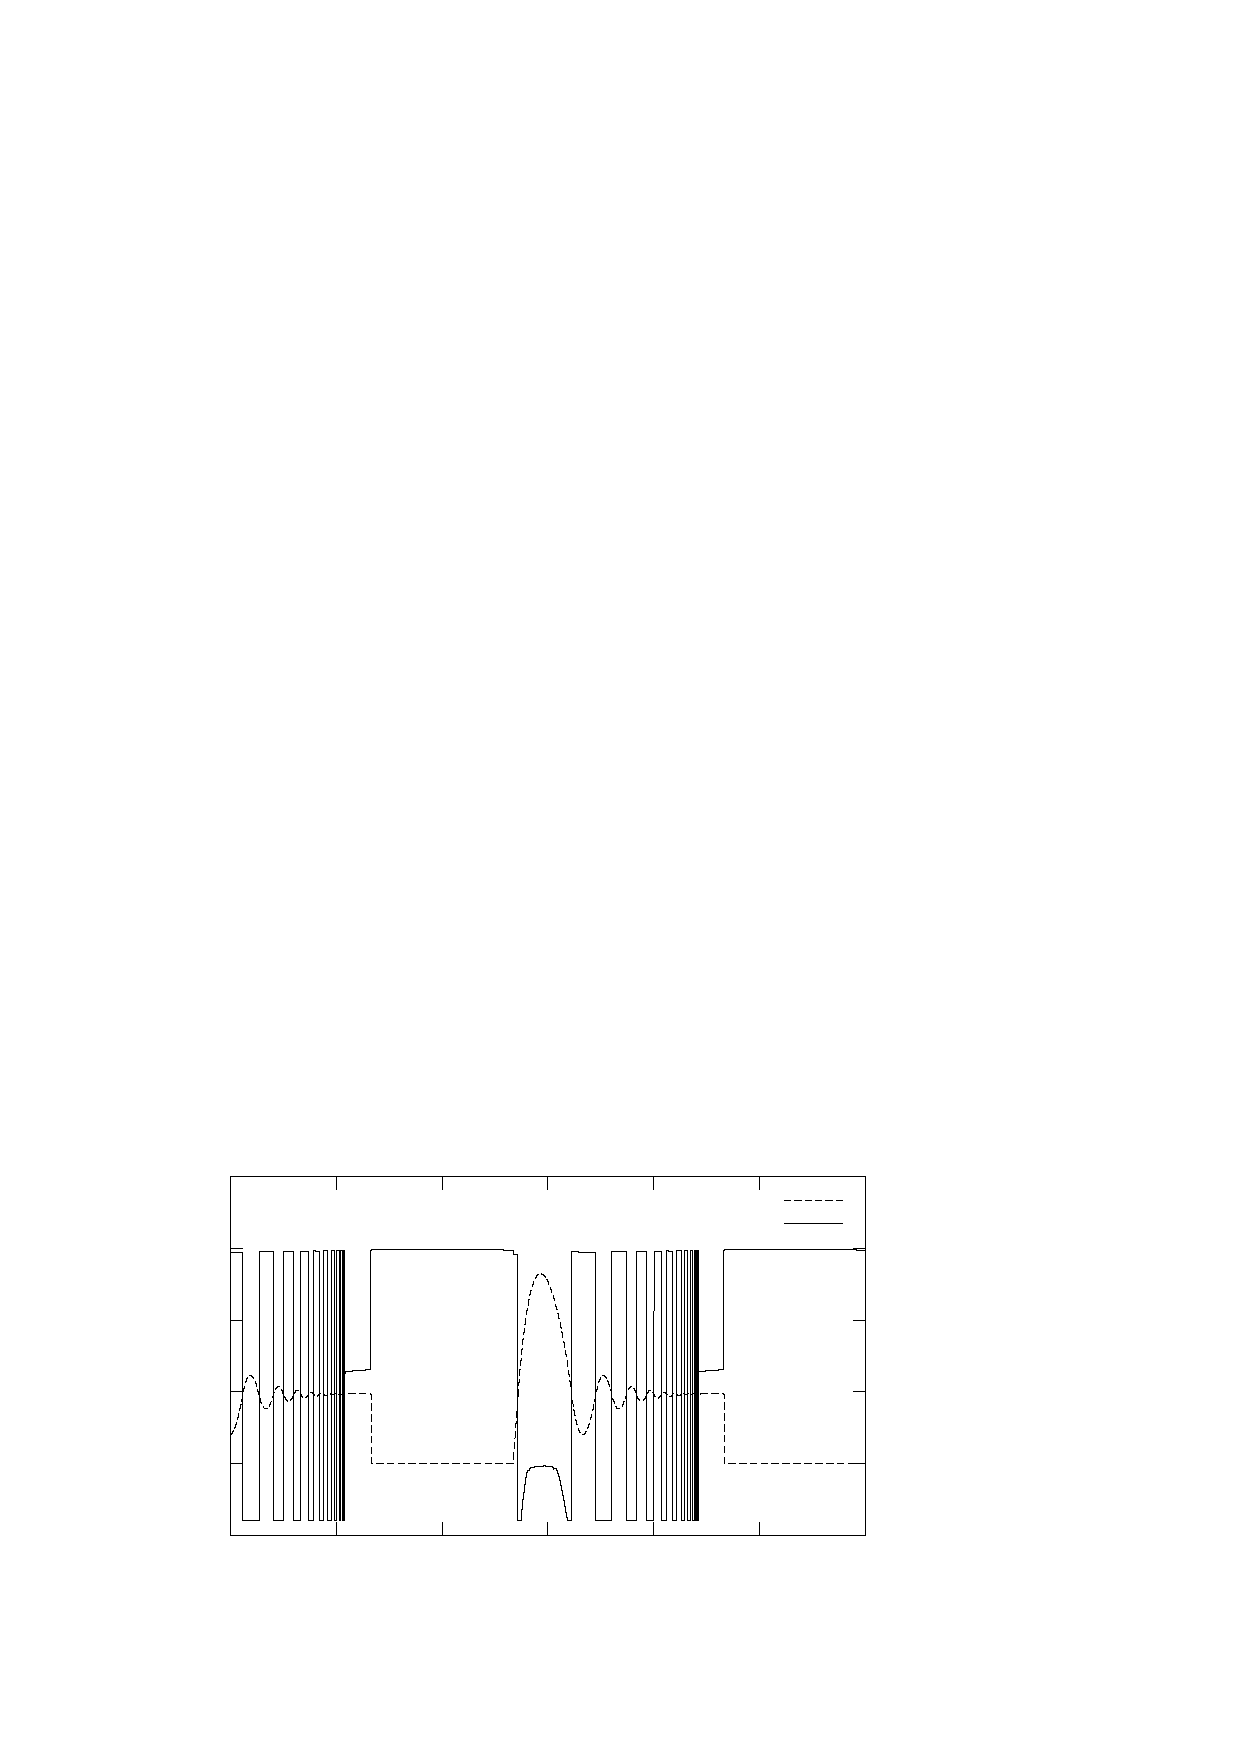
\includegraphics{VcompVdrainSliding}%
\end{picture}%
\begingroup
\setlength{\unitlength}{0.0200bp}%
\begin{picture}(18000,10800)(0,0)%
\put(1650,1650){\makebox(0,0)[r]{\strut{}-1}}%
\put(1650,3370){\makebox(0,0)[r]{\strut{} 0}}%
\put(1650,5090){\makebox(0,0)[r]{\strut{} 1}}%
\put(1650,6810){\makebox(0,0)[r]{\strut{} 2}}%
\put(1650,8530){\makebox(0,0)[r]{\strut{} 3}}%
\put(1650,10250){\makebox(0,0)[r]{\strut{} 4}}%
\put(1925,1100){\makebox(0,0){\strut{} 196}}%
\put(4467,1100){\makebox(0,0){\strut{} 196.5}}%
\put(7008,1100){\makebox(0,0){\strut{} 197}}%
\put(9550,1100){\makebox(0,0){\strut{} 197.5}}%
\put(12092,1100){\makebox(0,0){\strut{} 198}}%
\put(14633,1100){\makebox(0,0){\strut{} 198.5}}%
\put(17175,1100){\makebox(0,0){\strut{} 199}}%
\put(550,5950){\rotatebox{90}{\makebox(0,0){\strut{}V}}}%
\put(9550,275){\makebox(0,0){\strut{}time \micro s}}%
\put(14950,9675){\makebox(0,0)[r]{\strut{}$V_{comp}$}}%
\put(14950,9125){\makebox(0,0)[r]{\strut{}$V_{drain}$}}%
\end{picture}%
\endgroup
\endinput
}
  } \hspace{-2mm}
  \subfigure[$V_{ramp}$ and $V_{error}$ ]{\label{fig:SICONOS_SIMU_BUCK_SLIDING_VERROR}
        \resizebox{0.5\linewidth}{!}{%GNUPLOT: LaTeX picture with Postscript
\begin{picture}(0,0)%
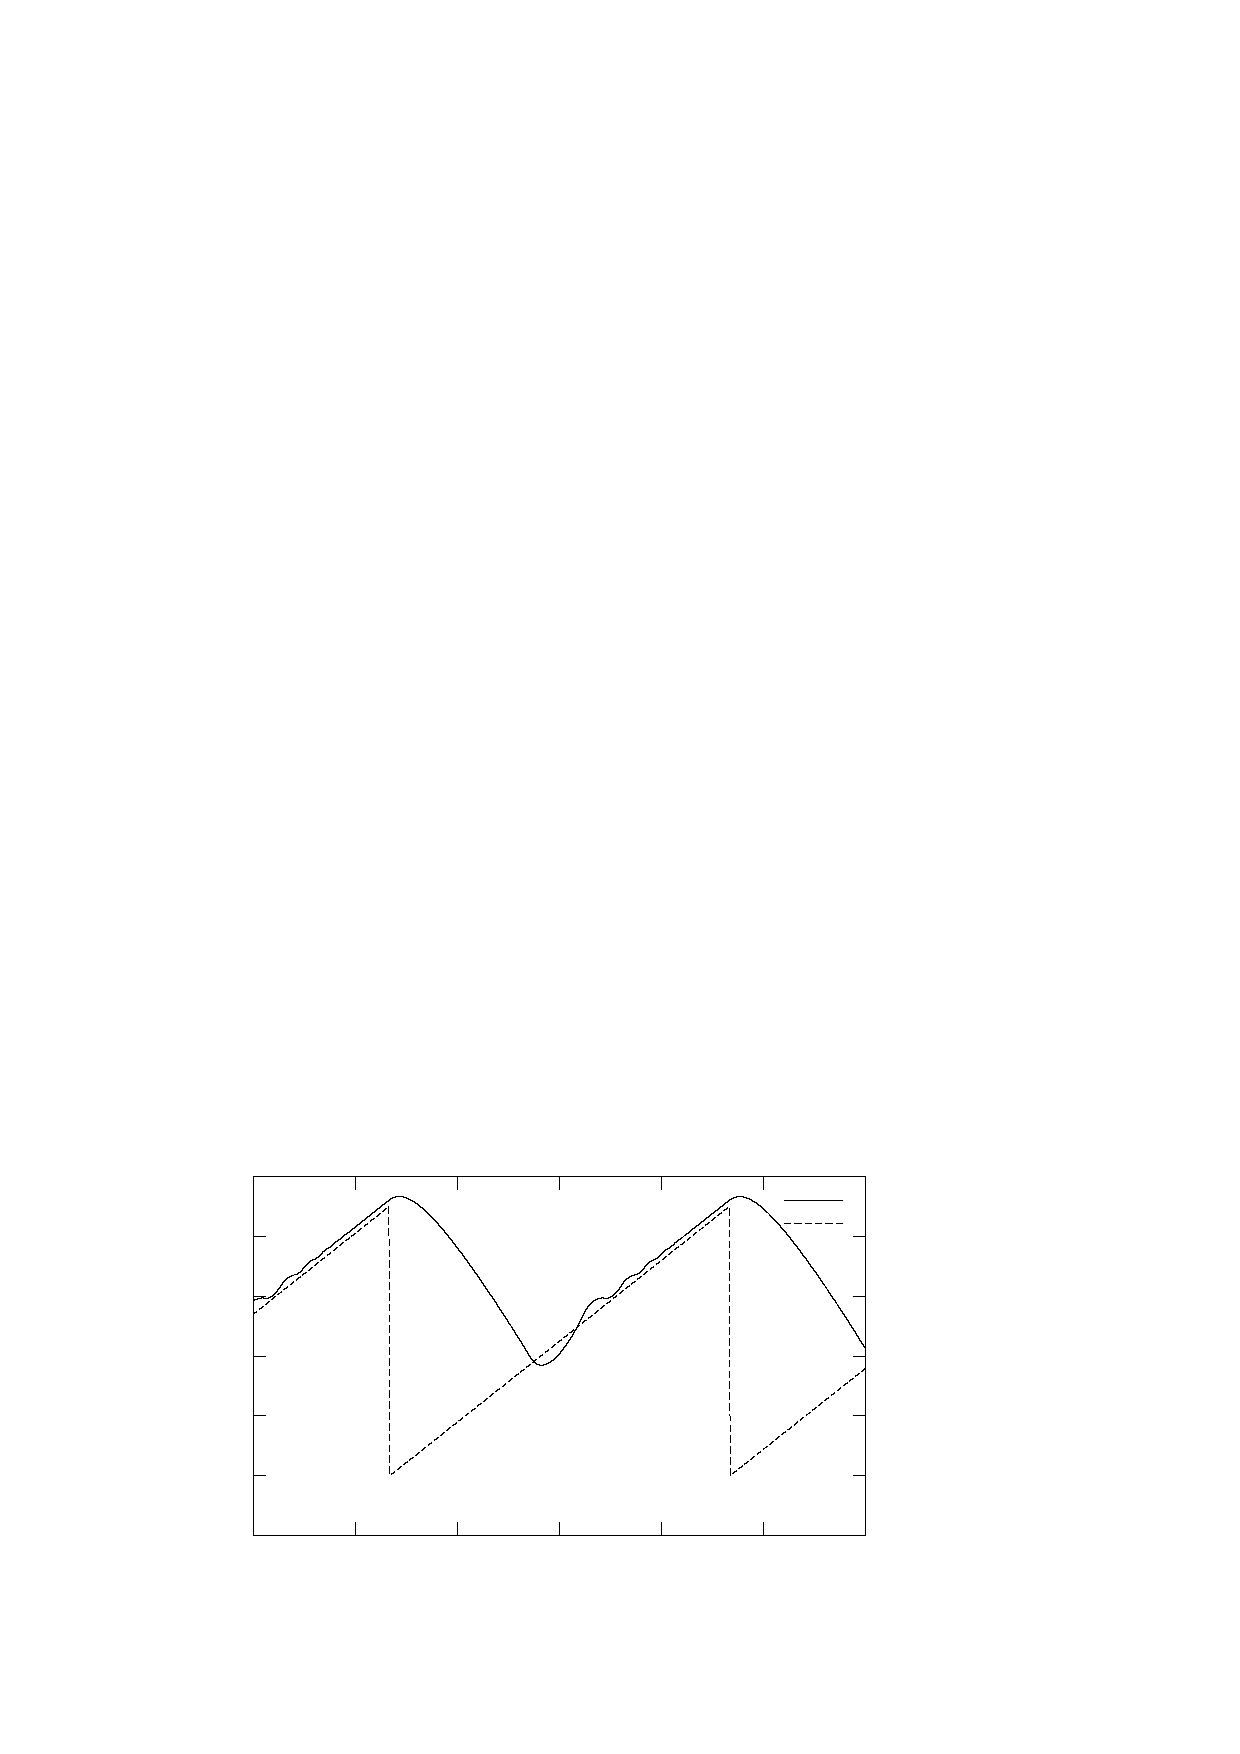
\includegraphics{VrampVerrorSliding}%
\end{picture}%
\begingroup
\setlength{\unitlength}{0.0200bp}%
\begin{picture}(18000,10800)(0,0)%
\put(2200,1650){\makebox(0,0)[r]{\strut{}-0.5}}%
\put(2200,3083){\makebox(0,0)[r]{\strut{} 0}}%
\put(2200,4517){\makebox(0,0)[r]{\strut{} 0.5}}%
\put(2200,5950){\makebox(0,0)[r]{\strut{} 1}}%
\put(2200,7383){\makebox(0,0)[r]{\strut{} 1.5}}%
\put(2200,8817){\makebox(0,0)[r]{\strut{} 2}}%
\put(2200,10250){\makebox(0,0)[r]{\strut{} 2.5}}%
\put(2475,1100){\makebox(0,0){\strut{} 196}}%
\put(4925,1100){\makebox(0,0){\strut{} 196.5}}%
\put(7375,1100){\makebox(0,0){\strut{} 197}}%
\put(9825,1100){\makebox(0,0){\strut{} 197.5}}%
\put(12275,1100){\makebox(0,0){\strut{} 198}}%
\put(14725,1100){\makebox(0,0){\strut{} 198.5}}%
\put(17175,1100){\makebox(0,0){\strut{} 199}}%
\put(550,5950){\rotatebox{90}{\makebox(0,0){\strut{}V}}}%
\put(9825,275){\makebox(0,0){\strut{}time \micro s}}%
\put(14950,9675){\makebox(0,0)[r]{\strut{}$V_{error}$}}%
\put(14950,9125){\makebox(0,0)[r]{\strut{}$V_{ramp}$}}%
\end{picture}%
\endgroup
\endinput
}
  }
  \caption{{\sc Siconos} buck simulation using sliding mode parameters.}
\label{fig:figSimuBuck_Sliding}
\end{figure*}


\begin{enumerate}
  \item[--] Fig.~\ref{fig:figSimuBuck} (a) is the output potential, following the ramp $V_{ref}$.
    \item[--] Fig.~\ref{fig:figSimuBuck} (b) is the current through the inductor. Until $0.0001s$, $I_L$
    is loading the capacitor C. After $0.0001s$, $I_L$ has to keep the capacitor charge constant.
    \item[--] Fig.~\ref{fig:figSimuBuck} (c) zooms on the pMOS drain potential with standard
    parameters.
    \item[--] Fig.~ \ref{fig:figSimuBuck} (d) zooms on the $V_{error}$ and $V_{ramp}$ voltages.
    \item[--] Fig.~ \ref{fig:figSimuBuck_Sliding} (a) using sliding mode parameters, shows the stabilization of the comparator output to an unsaturated value. It also shows
      the stabilization of the current through the pMOS allowing the $V_{error}$ signal to follow the $V_{ramp}$
    signal.    
    \item[--] Fig.~\ref{fig:figSimuBuck_Sliding} (b) using sliding mode parameters, shows the $V_{error}$ and $V_{ramp}$ voltages.
  \end{enumerate}




The simulation has been tested with many parameters values. The robustness of the nonsmooth
modelling and solving algorithms enables one to perform with the same CPU time the simulation of such cases.  



\subsubsection{Simulation with {\sc Spice} }

\paragraph{Simulation conditions: convergence issues related to the MOS model}
The simulation of this circuit was done with several versions of {\sc Spice} (the open source {\sc Ngspice} from
Berkeley and
{\sc Eldo} from Mentor Graphics) and two kinds of MOS models :
\begin{description}
\item \textbf{The MOS level 3 model :}  This model takes more physical effects into account than the piecewise-linear model used in {\sc Siconos} simulations,
in particular the voltage-dependent capacitances. It is an important issue since these varying capacitances
cause some convergence problems when node 2 switches between $V_I$ and ground.
Adding a small capacitor of a few picoFarad between this node and ground helps to solve the problem
but may yield artifacts (spikes) on the current of the~$V_I$~alim and the MOS transistors.
\item\textbf{An nMOS simplified model (Sah model)} with fixed capacitances and a quadratic static characteristic :
\[
I_{DS} = \textrm{max}(0,V_{GS}-Vt_N)^2 - \textrm{max}(0,V_{GD}-Vt_N)^2 
\]
This model is very close to the piecewise-linear model used in {\sc Siconos} simulations. The implementation in netlists was done thanks to 
voltage-dependent current sources that are very likely not compiled by the various {\sc Spice} simulators tested.
Thus the measured CPU time is increased with respect to a compiled version.
An estimation of the CPU time with a compiled simplified model may be  given by multiplying the MOS level 3 CPU time
by the ratio of the Newton-Raphson iterations required respectively during the simulations with each model.
An additional correction should be done to reflect that the computation of the jacobian matrix entries
linked to a compiled simplified model would require less time than with a MOS level 3 model. Even if the {\sc Spice} simulation
includes other operations, jacobian matrix loading time is indeed known to be generally predominant.
\end{description}


\begin{itemize}
\item Power MOSFETS intrinsic diodes are modelled by the classical Shockley equation with an emission
coefficient $N~=~1$ :
\[ I = I_S.({e^{\frac{q.V}{N.k.T}} - 1}) \qquad \textrm{when} \quad V > -5.N.\frac{k.T}{q} \]
\[ I = -I_S \qquad  \textrm{when} \quad V < -5.N.\frac{k.T}{q} \]
with $V\,,\,I $ voltage and current through the diode,  $I_S$ saturation current, default value $10^{-14}$~A, $q$electron charge $1.6\,10^{-19}$~C, $k$ Boltzmann constant $1.38\,10^{-23}\,J.K^{-1}$, $T$ temperature in K and $N$ emission coefficient.
\item The comparator is modelled as a non linear voltage controlled voltage source defined as $V_{out}~=~1.5(\tanh(10V_{in}) + 1)$. Thus the 3-segment characteristic used as the nonsmooth model is regularized to help convergence of {\sc Spice}
(see a comparison of the piecewise-linear comparator as used in {\sc Siconos} simulations with the {\sc Spice} one on Fig.~\ref{fig-comparator-models}).
\end{itemize}

\begin{figure}[hbtp]
\begin{center}
%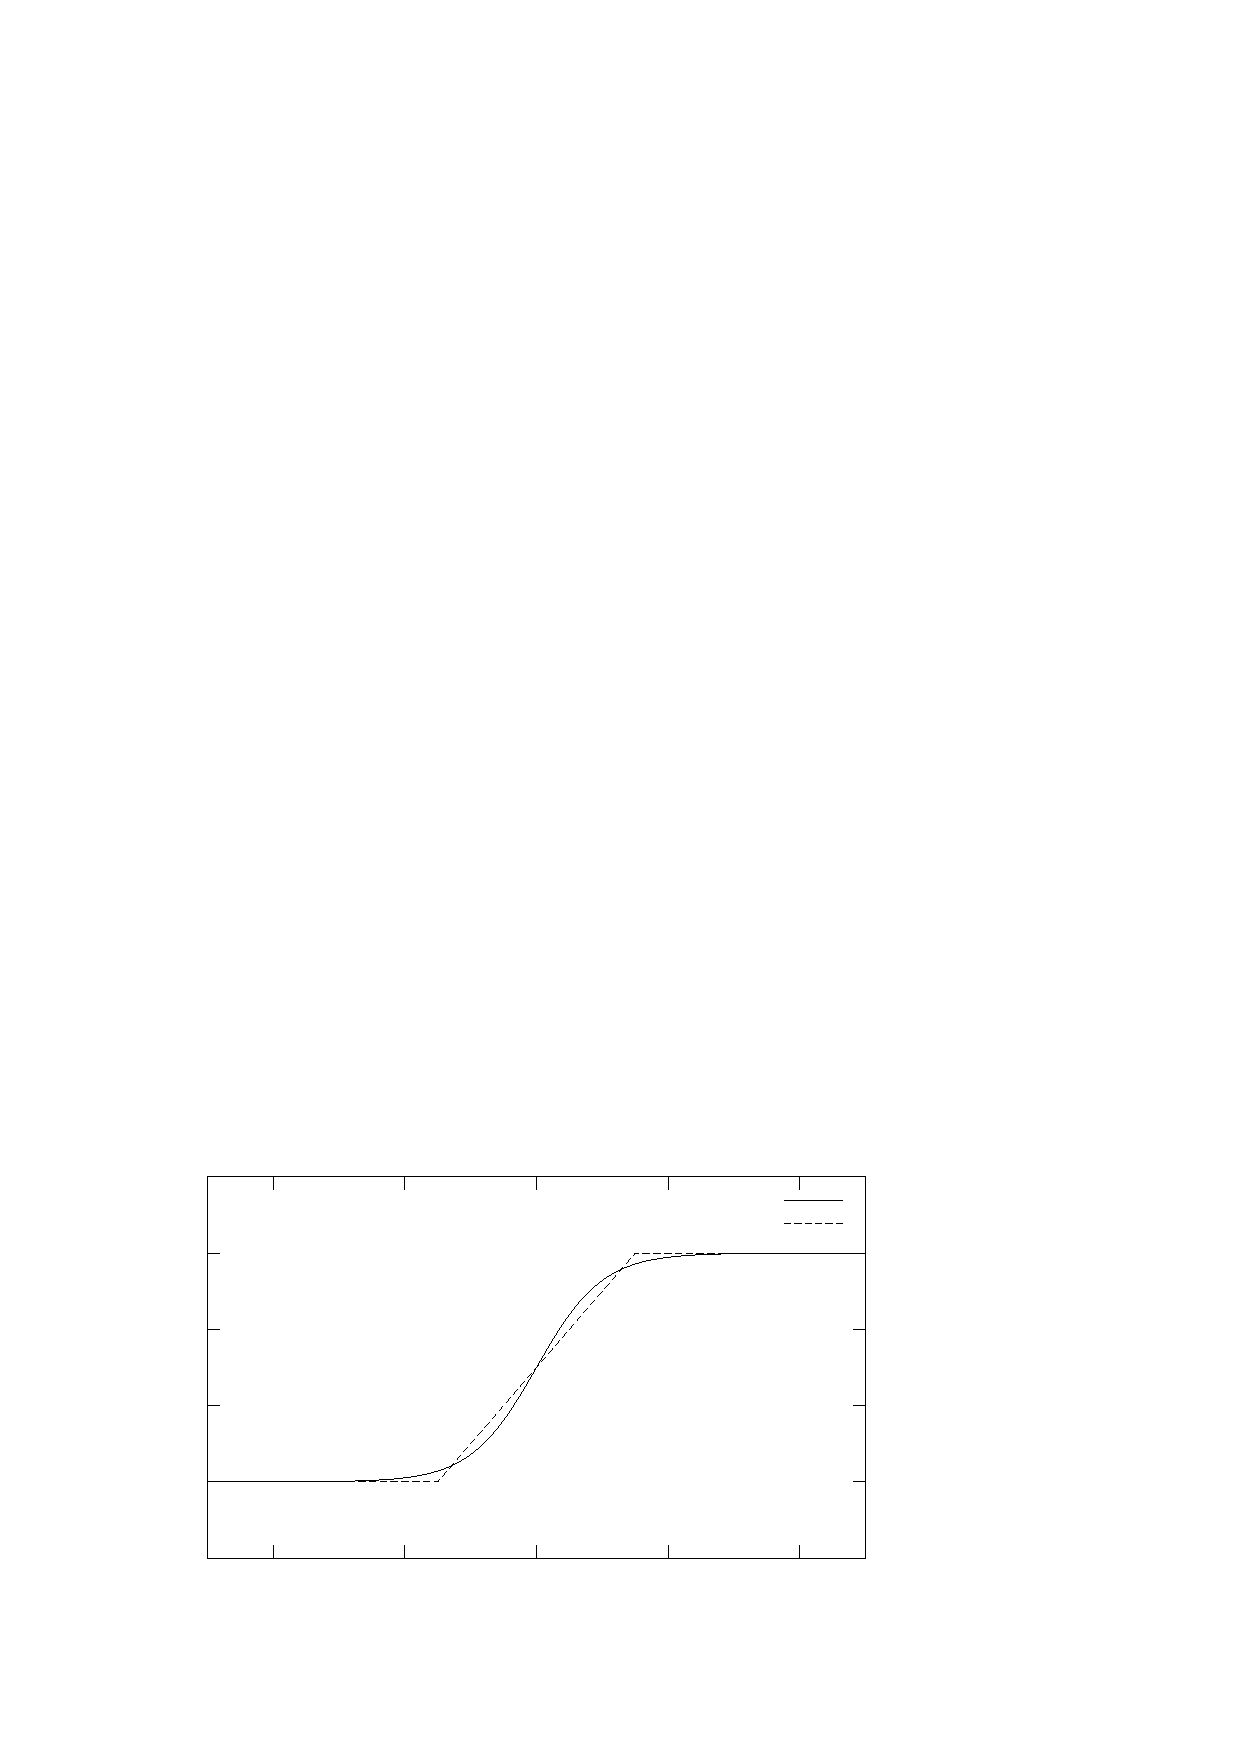
\includegraphics[scale=0.6,angle=0]{./figure/tanh_pwl.tex}
  \resizebox{\linewidth}{!}{
  %GNUPLOT: LaTeX picture with Postscript
\begin{picture}(0,0)%
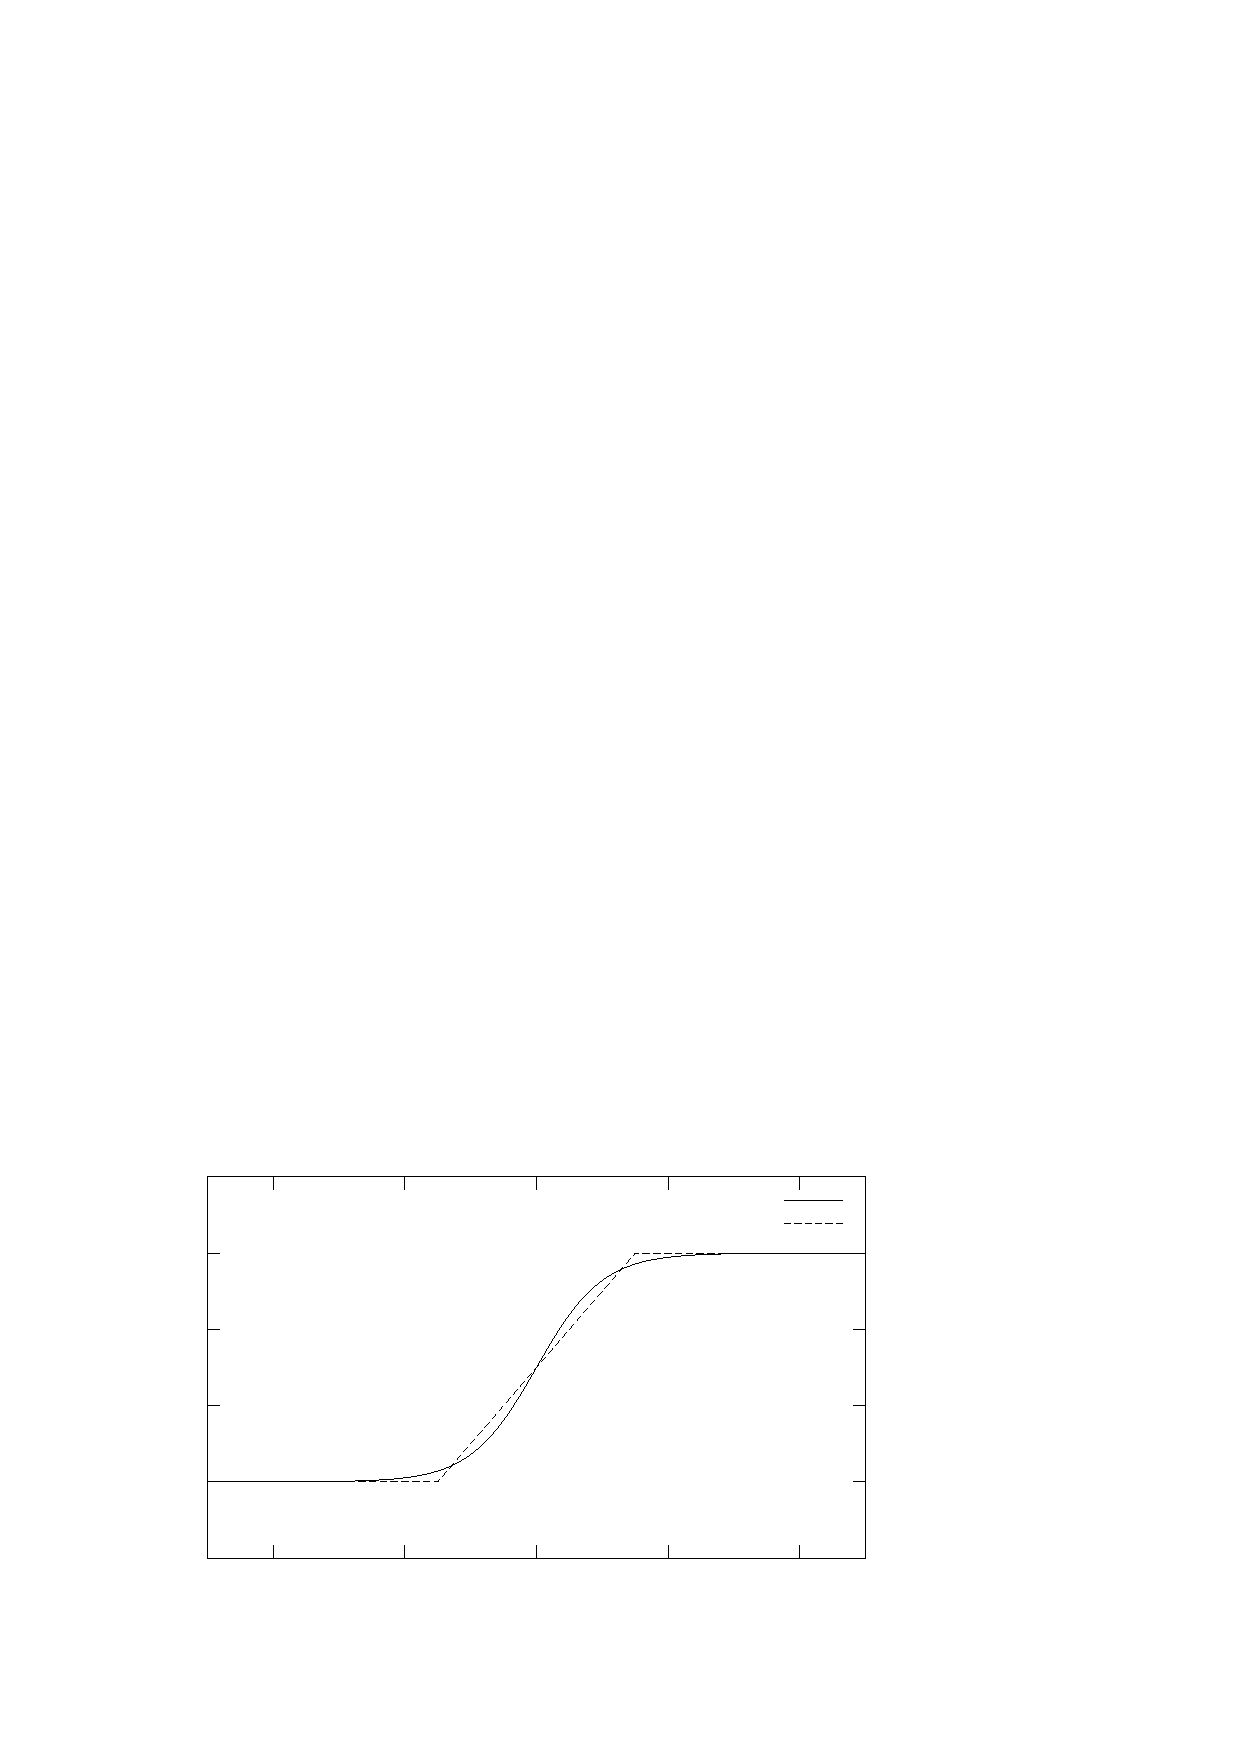
\includegraphics{tanh_pwl}%
\end{picture}%
\begingroup
\setlength{\unitlength}{0.0200bp}%
\begin{picture}(18000,10800)(0,0)%
\put(1100,1100){\makebox(0,0)[r]{\strut{}-1}}%
\put(1100,2930){\makebox(0,0)[r]{\strut{} 0}}%
\put(1100,4760){\makebox(0,0)[r]{\strut{} 1}}%
\put(1100,6590){\makebox(0,0)[r]{\strut{} 2}}%
\put(1100,8420){\makebox(0,0)[r]{\strut{} 3}}%
\put(1100,10250){\makebox(0,0)[r]{\strut{} 4}}%
\put(2955,550){\makebox(0,0){\strut{}-0.4}}%
\put(6115,550){\makebox(0,0){\strut{}-0.2}}%
\put(9275,550){\makebox(0,0){\strut{} 0}}%
\put(12435,550){\makebox(0,0){\strut{} 0.2}}%
\put(15595,550){\makebox(0,0){\strut{} 0.4}}%
\put(14950,9675){\makebox(0,0)[r]{\strut{}ftanh(x)}}%
\put(14950,9125){\makebox(0,0)[r]{\strut{}fpwl(x)}}%
\end{picture}%
\endgroup
\endinput
}
\end{center}{Comparison of piecewise-linear and {\sc Spice} ($\tanh$ based) comparator models.}
\label{fig-comparator-models}
\end{figure}



The power supply $V_I$ is raised from 0 in $50~\nano\second$ at the beginning to help the convergence.\footnote{This is
not required with the {\sc Siconos} algorithms that find a consistent initial solution from scratch.}
The {\sc Spice} tolerance values used are $1\nano\ampere$ for currents, $1\micro\volt$ for voltages and $0.00075$ for relative differences.
The maximum number of Newton-Raphson iterations is set to $100$ (the default values are $10$ for
{\sc Ngspice} and $13$ for {\sc Eldo}).

Usually, {\sc Spice} simulators integrate with a time step adjusted according to different strategies based on an estimation
of the local truncation error (LTE) or the number of Newton-Raphson iterations required by previous steps.
Since {\sc Siconos} simulations were carried with a fixed time step of~50~ps, simulators were forced to use this value as a maximum.
Even when {\sc Spice} simulators use a fixed time step, they may compute LTE to assess a solution found by the Newton-Raphson
algorithm. This computation of LTE was disabled because it could impair the performance of {\sc Spice} with respect to {\sc Siconos}.
\footnote{For {\sc Ngspice}, it implied a slight modification of the source code since no standard option is provided to do it.}

\subsubsection{Simulation comparisons}
The table \ref{tab:buck} displays the results with the standard and the sliding mode values of compensator components. An estimation of the CPU time with a compiled simplified model is added.
\\
\\
\begin{table}
  \centering
  \begin{tabular}{|l|c|r|r|}
\hline
simulator & model &
%begin{tabular}{c}
{ \# Newton  iterations}
%\end{tabular}
&
%\begin{tabular}{c}
{ CPU  time (s)}
%\end{tabular}
\\
\hline
\multicolumn{4}{|c|}{\textbf{standard compensator values}}\\
\hline
{\sc Ngspice} & simple   & 8024814 & 632 \\
{\sc Ngspice} & level 3  & 8304237 & 370 \\
\hline
%SMASH   & simple  & 4000404 & 8073070 & 230 \\
%SMASH   & level 3 & 4000323 & 8059868 & 172 \\
%\hline
{\sc Eldo}    & simple   & 4547579 & 388 \\
{\sc Eldo}    & level 3  & 4554452 & 356 \\
\hline
{\sc Siconos}    & LCP   & --  & 60 \\
\hline
\multicolumn{4}{|c|}{\textbf{sliding mode compensator values}}\\
\hline
{\sc Ngspice} & simple   & 8070324 & 638 \\
{\sc Ngspice} & level 3  & 8669053 & 385 \\
\hline
%SMASH   & simple  & 4000252 & 8239697 & 234 \\
%SMASH   & level 3 & 4000131 & 8220181 & 176 \\
%\hline
{\sc Eldo}    & simple   & 5861226 & 438 \\
{\sc Eldo}    & level 3  & 5888994 & 367 \\
\hline
{\sc Siconos}    & LCP   & -- & 60 \\
\hline
\end{tabular}\\
\caption{Numerical comparison on the Buck converter Example}
\label{tab:buck}
\end{table}
\\
\\
These results shall be compared to the 60~s~CPU time achieved with the NSDS method.
Depending on the model and the {\sc Spice} simulator, the (estimated) CPU time is from~2.8~to~6.1
larger than with {\sc Siconos}. Moreover, it was necessary to add a parasitic capacitor on the connection between the pMOS and nMOS
transistors to allow the convergence of the {\sc Ngspice} simulator with the MOS level 3 model. All the {\sc Siconos} simulations
presented in this paper have been obtained in one-shot from the dynamical equations automatically
generated from the Netlist, without any further parameter tuning.

\subsubsection{Sliding mode using a multi-valued comparator}
\begin{figure*}[!ht]
    \subfigure[$V_{comp}$ and $V_{drain}$]  
  {\label{fig:SICONOS_SIMU_BUCK_SLIDING_MV_MOS_COMP} 
        \resizebox{0.5\linewidth}{!}{%GNUPLOT: LaTeX picture with Postscript
\begin{picture}(0,0)%
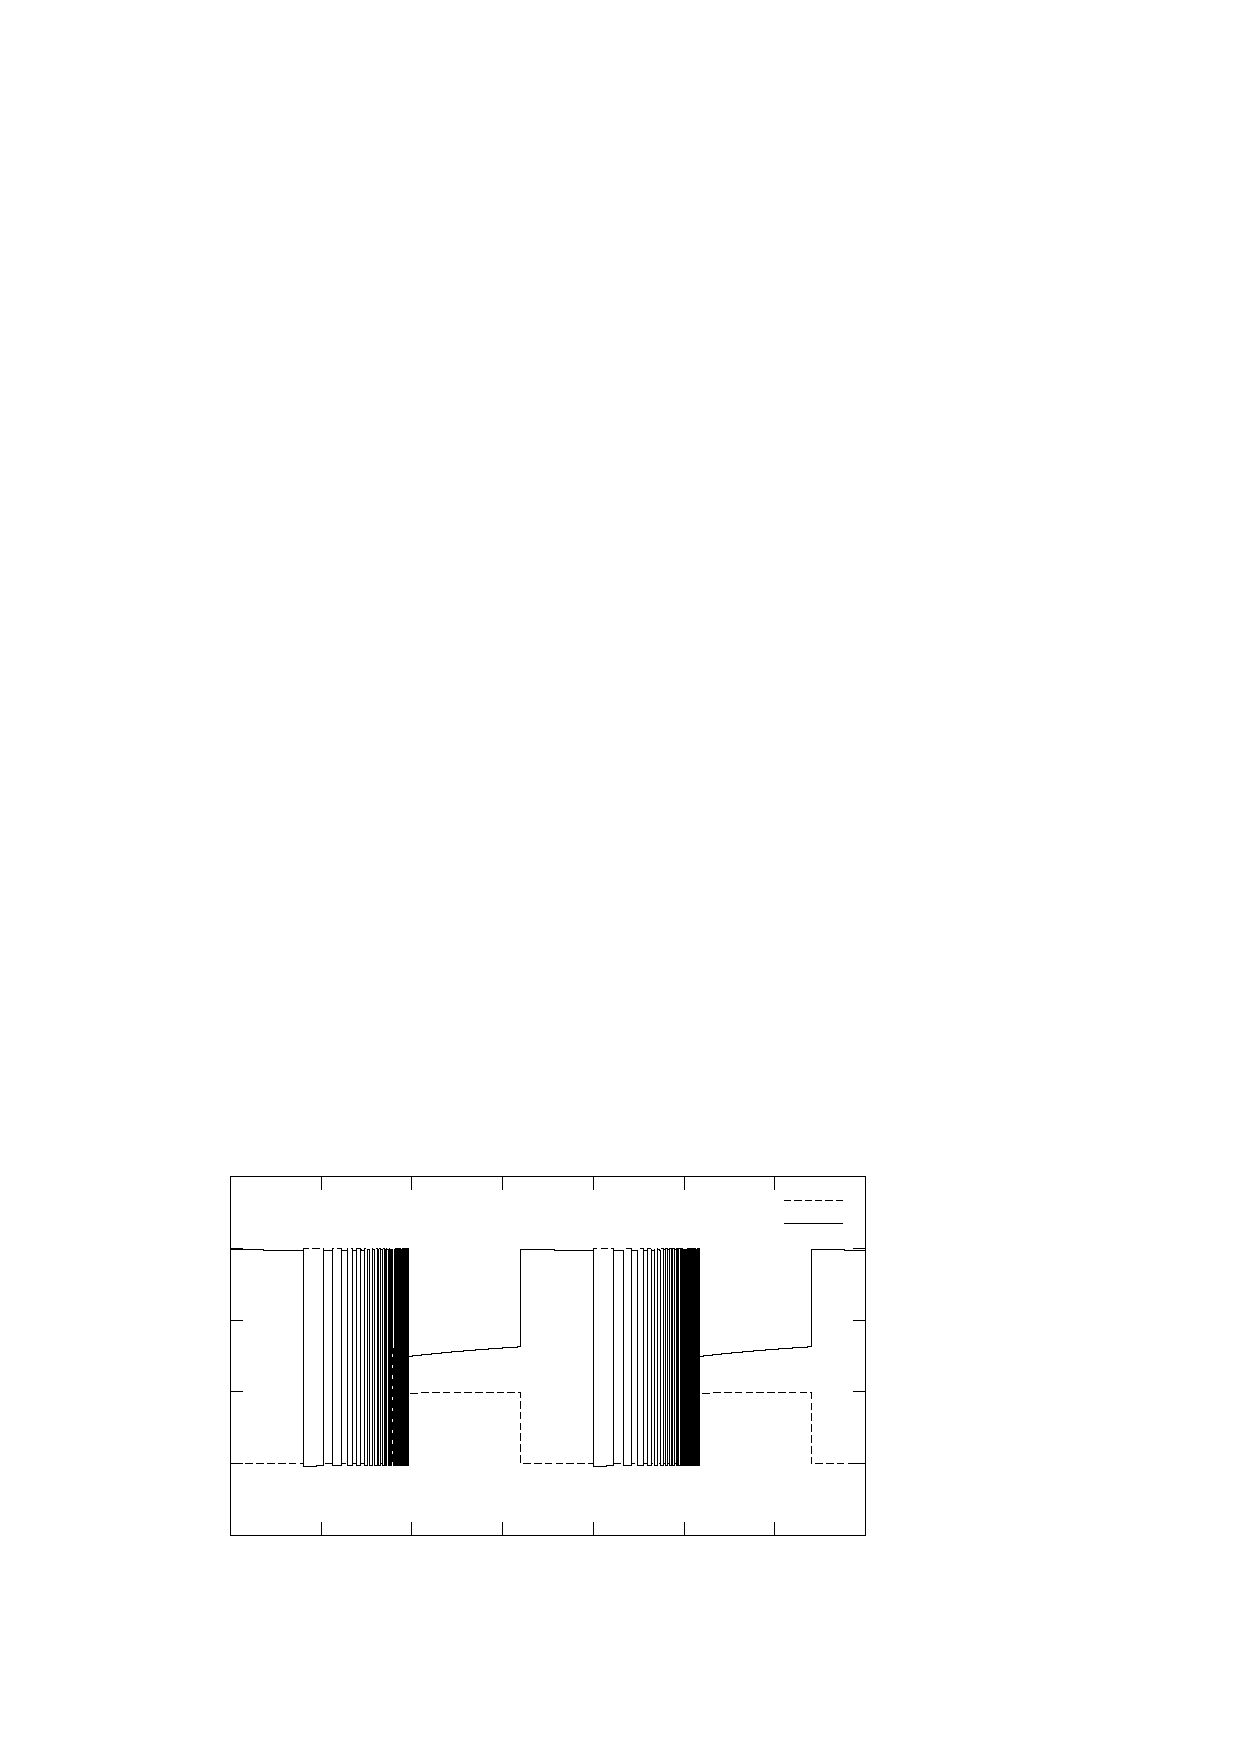
\includegraphics{VcompVdrainSliding_mv}%
\end{picture}%
\begingroup
\setlength{\unitlength}{0.0200bp}%
\begin{picture}(18000,10800)(0,0)%
\put(1650,1650){\makebox(0,0)[r]{\strut{}-1}}%
\put(1650,3370){\makebox(0,0)[r]{\strut{} 0}}%
\put(1650,5090){\makebox(0,0)[r]{\strut{} 1}}%
\put(1650,6810){\makebox(0,0)[r]{\strut{} 2}}%
\put(1650,8530){\makebox(0,0)[r]{\strut{} 3}}%
\put(1650,10250){\makebox(0,0)[r]{\strut{} 4}}%
\put(1925,1100){\makebox(0,0){\strut{} 192}}%
\put(4104,1100){\makebox(0,0){\strut{} 193}}%
\put(6282,1100){\makebox(0,0){\strut{} 194}}%
\put(8461,1100){\makebox(0,0){\strut{} 195}}%
\put(10639,1100){\makebox(0,0){\strut{} 196}}%
\put(12818,1100){\makebox(0,0){\strut{} 197}}%
\put(14996,1100){\makebox(0,0){\strut{} 198}}%
\put(17175,1100){\makebox(0,0){\strut{} 199}}%
\put(550,5950){\rotatebox{90}{\makebox(0,0){\strut{}V}}}%
\put(9550,275){\makebox(0,0){\strut{}time \micro s}}%
\put(14950,9675){\makebox(0,0)[r]{\strut{}$V_{comp}$}}%
\put(14950,9125){\makebox(0,0)[r]{\strut{}$V_{drain}$}}%
\end{picture}%
\endgroup
\endinput
}
  } \hspace{-2mm}
  \subfigure[$V_{ramp}$ and $V_{error}$ ]{\label{fig:SICONOS_SIMU_BUCK_SLIDING_VERROR_MV}
        \resizebox{0.5\linewidth}{!}{\input{./figure/VrampVerrorSlidingMV.pstex_t }}
  }
  \caption{{\sc Siconos} buck simulation using sliding mode parameters and multivalued comparator.}
\label{fig:figSimuBuck_Sliding_mv}
\end{figure*}

\begin{figure*}[!ht]
    \subfigure[$V_{comp}$ and $V_{drain}$]  
  {\label{fig:ELDO_SIMU_BUCK_SLIDING_MV_MOS_COMP} 
        \resizebox{0.5\linewidth}{!}{\input{./figure/VcompVdrainSlidingMV_eldo.pstex_t}}
  } \hspace{-2mm}
  \subfigure[$V_{ramp}$ and $V_{error}$ ]{\label{fig:ELDO_SIMU_BUCK_SLIDING_VERROR}
        \resizebox{0.5\linewidth}{!}{\input{./figure/VrampVerrorSlidingMV_eldo.pstex_t }}
  }
  \caption{{\sc Eldo} buck simulation using sliding mode parameters and $V_{out}~=~1.5(\tanh(10000 V_{in}) + 1)$ for the comparator.}
\label{fig:figSimuBuck_Sliding_mv_eldo}
\end{figure*}
This paragraph focuses on the simulation with sliding parameters and using a multi-valued model for the comparator. The rise
time of the ramp voltage has been increased to $3.2 \nano \second$. The model used in {\sc Siconos}
consists in setting the $\epsilon$ gap to $0$ in the model depicted in ~\ref{eq_MV_comp}. Fig.
~\ref{fig:figSimuBuck_Sliding_mv} shows the {\sc Siconos} simulation using a fully implicit time-stepping. It could be noted that
the comparator output is stabilized to an unsaturated value. Simulation using {\sc Eldo} has been
done using the model $V_{out}~=~1.5(\tanh(10000 V_{in}) + 1)$ for the comparator. The MOS
level 3 leads to 'Newton no-convergence' messages, so the MOS SAh model has been used to run the simulation displayed in Fig.~\ref{fig:figSimuBuck_Sliding_mv_eldo}.
It is noteworthy that it does not handle the stabilization of the comparator output on the sliding surface. 





\subsubsection{Simulation with {\sc Plecs}}

As we pointed out above, the hybrid approach that consists of an exhaustive enumeration of all the
system's modes, soon become inefficient and unusable mainly because the simulation duration grows
exponentially fast. Let us illustrate this fact with the buck converter, loaded with several
devices: a resistance, and a chain of transistors. The simulator is {\sc Plecs}, a hybrid simulator developed by Plexim \footnote{http://www.plexim.com/}. 

The CPU time required to achieve the simulation of $200 \micro\second$ ranges between $596 \second$ to $4$ hours,
depending on the values of the resistors, capacitors and inductors and the existence of sliding modes. This should be compared to the
$60\second$ of the {\sc Siconos} simulation, obtained independently of these components values.
Moreover, the {\sc Plecs} simulation performs only $168038$ steps comparing the $4.10^{6}$ steps performed during the {\sc Siconos}
simulation. It can be concluded that the computation of one step of simulation using {\sc Siconos} is $250$
faster than using {\sc Plecs}. This demonstrates the robustness and efficiency of the time-stepping scheme
and the OSNSP algorithms of {\sc Siconos}.

\begin{remark}
  On both Fig.\ref{fig:SICONOS_SIMU_BUCK_SLIDING_MV_MOS_COMP} and Fig.~\ref{fig:SICONOS_SIMU_BUCK_SLIDING_VERROR} it is seen that the sliding surface is attained in
  finite time after an accumulation of switches. This is a classical phenomenon in nonsmooth
  systems, see Filippov's example in \cite{Acary.Brogliato2009}.
\end{remark}
\section{Conclusions}
\label{section5}


In this paper we have presented numerical simulations of switched circuits obtained with a suitable time-stepping implicit method, named Moreau's time-stepping algorithm. This method is based on the nonsmooth dynamical systems modelling approach, and relies heavily on complementarity problems (equivalently, inclusions into normal cones) solvers. The advantages of such a method are that it allows one to:

\begin{itemize}

\item avoid computing the dynamics changes due to topology variations, since the circuits are treated as a global system with a fixed state dimension; modes transitions are taken care of by the complementarity problem solvers, which usually are polynomial in time;

\item simulate circuits with very large number of events without slowing down too much the simulation;

\item avoid regularization and consequently stiff systems of ODEs;

\item accurately calculate the initial steady-state of the system;

\item accurately simulate sliding mode trajectories without spurious oscillations around the switching surface;

\item compute state jumps (initial jumps due to inconsistent states, or in the course of the integration). 

\end{itemize}


The major drawback of the used method is its low order, so that its accuracy may be less good on smooth portions of the trajectoires. In this paper it is first shown that Moreau's time-stepping scheme allows one to integrate an academic example on which Newton-Raphson based methods fail. Then the buck converter system is simulated. Comparisons with other analog simulators are presented. The simulations have been led with the {\sc Siconos} software package of the INRIA, an open source platform dedicated to nonsmooth multivalued dynamical systems. 




%%% Local Variables: 
%%% mode: latex
%%% TeX-master: "IEEEpaper"
%%% End: 
